% !TeX root = ../main.tex

\chapter{核心章节}
\label{cha:3}
\section{tikz绘图}
\par tikz\footnote{\url{http://mirrors.ctan.org/graphics/pgf/base/doc/pgfmanual.pdf}}是latex的绘图宏包,建议参考YunYouJun大佬硕士论文模板\url{https://github.com/YunYouJun/cucthesis}里的绘制方式,其生成的pdf在\url{https://yunyoujun.github.io/cucthesis/}。
\section{插入plantuml绘图}
\par plantuml\footnote{\url{https://plantuml.com/}}可以快速绘制多种图表,如时序\cref{fig:plantuml_tex},环境配置与操作详见README.md。
\subsection{方案一:直接导出tex插入(推荐)}
\begin{figure}[htbp]
    \centering
    \resizebox{0.8\textwidth}{!}{% generated by Plantuml 1.2023.5       
\definecolor{plantucolor0000}{RGB}{24,24,24}
\definecolor{plantucolor0001}{RGB}{226,226,240}
\definecolor{plantucolor0002}{RGB}{0,0,0}
\begin{tikzpicture}[yscale=-1
,pstyle0/.style={color=plantucolor0000,line width=0.5pt,dash pattern=on 5.0pt off 5.0pt}
,pstyle1/.style={color=plantucolor0000,fill=plantucolor0001,line width=0.5pt}
,pstyle2/.style={color=plantucolor0000,line width=0.5pt}
,pstyle3/.style={color=plantucolor0000,fill=plantucolor0000,line width=1.0pt}
,pstyle4/.style={color=plantucolor0000,fill=plantucolor0001,line width=1.5pt}
,pstyle5/.style={color=plantucolor0000,line width=1.5pt}
,pstyle6/.style={color=plantucolor0000,line width=1.0pt}
]
\draw[pstyle0] (47pt,82.7461pt) -- (47pt,316.0957pt);
\draw[pstyle0] (122.5431pt,82.7461pt) -- (122.5431pt,316.0957pt);
\draw[pstyle0] (189.5681pt,82.7461pt) -- (189.5681pt,316.0957pt);
\draw[pstyle0] (262.0718pt,82.7461pt) -- (262.0718pt,316.0957pt);
\draw[pstyle0] (322.9003pt,82.7461pt) -- (322.9003pt,316.0957pt);
\draw[pstyle0] (389.2579pt,82.7461pt) -- (389.2579pt,316.0957pt);
\draw[pstyle0] (477.9873pt,82.7461pt) -- (477.9873pt,316.0957pt);
\draw[pstyle0] (565.8712pt,82.7461pt) -- (565.8712pt,316.0957pt);
\draw[pstyle1] (5pt,55pt) arc (180:270:5pt) -- (10pt,50pt) -- (84.8pt,50pt) arc (270:360:5pt) -- (89.8pt,55pt) -- (89.8pt,76.7461pt) arc (0:90:5pt) -- (84.8pt,81.7461pt) -- (10pt,81.7461pt) arc (90:180:5pt) -- (5pt,76.7461pt) -- cycle;
\node at (12pt,57pt)[below right,color=black]{Participant};
\draw[pstyle1] (5pt,320.0957pt) arc (180:270:5pt) -- (10pt,315.0957pt) -- (84.8pt,315.0957pt) arc (270:360:5pt) -- (89.8pt,320.0957pt) -- (89.8pt,341.8418pt) arc (0:90:5pt) -- (84.8pt,346.8418pt) -- (10pt,346.8418pt) arc (90:180:5pt) -- (5pt,341.8418pt) -- cycle;
\node at (12pt,322.0957pt)[below right,color=black]{Participant};
\node at (100.5431pt,65pt)[below right,color=black]{Actor};
\draw[pstyle1] (122.5556pt,13.5pt) ellipse (8pt and 8pt);
\draw[pstyle2] (122.5556pt,21.5pt) -- (122.5556pt,48.5pt)(109.5556pt,29.5pt) -- (135.5556pt,29.5pt)(122.5556pt,48.5pt) -- (109.5556pt,63.5pt)(122.5556pt,48.5pt) -- (135.5556pt,63.5pt);
\node at (100.5431pt,315.0957pt)[below right,color=black]{Actor};
\draw[pstyle1] (122.5556pt,341.3418pt) ellipse (8pt and 8pt);
\draw[pstyle2] (122.5556pt,349.3418pt) -- (122.5556pt,376.3418pt)(109.5556pt,357.3418pt) -- (135.5556pt,357.3418pt)(122.5556pt,376.3418pt) -- (109.5556pt,391.3418pt)(122.5556pt,376.3418pt) -- (135.5556pt,391.3418pt);
\node at (154.5681pt,65pt)[below right,color=black]{Boundary};
\draw[pstyle2] (169.3199pt,37pt) -- (169.3199pt,61pt)(169.3199pt,49pt) -- (186.3199pt,49pt);
\draw[pstyle1] (198.3199pt,49pt) ellipse (12pt and 12pt);
\node at (154.5681pt,315.0957pt)[below right,color=black]{Boundary};
\draw[pstyle2] (169.3199pt,336.8418pt) -- (169.3199pt,360.8418pt)(169.3199pt,348.8418pt) -- (186.3199pt,348.8418pt);
\draw[pstyle1] (198.3199pt,348.8418pt) ellipse (12pt and 12pt);
\node at (235.0718pt,65pt)[below right,color=black]{Control};
\draw[pstyle1] (262.986pt,49pt) ellipse (12pt and 12pt);
\draw[pstyle3] (258.986pt,37pt) -- (264.986pt,32pt) -- (262.986pt,37pt) -- (264.986pt,42pt) -- (258.986pt,37pt) -- cycle;
\node at (235.0718pt,315.0957pt)[below right,color=black]{Control};
\draw[pstyle1] (262.986pt,348.8418pt) ellipse (12pt and 12pt);
\draw[pstyle3] (258.986pt,336.8418pt) -- (264.986pt,331.8418pt) -- (262.986pt,336.8418pt) -- (264.986pt,341.8418pt) -- (258.986pt,336.8418pt) -- cycle;
\node at (300.9003pt,65pt)[below right,color=black]{Entity};
\draw[pstyle1] (323.5791pt,49pt) ellipse (12pt and 12pt);
\draw[pstyle2] (311.5791pt,63pt) -- (335.5791pt,63pt);
\node at (300.9003pt,315.0957pt)[below right,color=black]{Entity};
\draw[pstyle1] (323.5791pt,348.8418pt) ellipse (12pt and 12pt);
\draw[pstyle2] (311.5791pt,362.8418pt) -- (335.5791pt,362.8418pt);
\node at (356.2579pt,65pt)[below right,color=black]{Database};
\draw[pstyle4] (371.6226pt,29pt) ..controls (371.6226pt,19pt) and (389.6226pt,19pt) .. (389.6226pt,19pt) ..controls (389.6226pt,19pt) and (407.6226pt,19pt) .. (407.6226pt,29pt) -- (407.6226pt,55pt) ..controls (407.6226pt,65pt) and (389.6226pt,65pt) .. (389.6226pt,65pt) ..controls (389.6226pt,65pt) and (371.6226pt,65pt) .. (371.6226pt,55pt) -- (371.6226pt,29pt);
\draw[pstyle5] (371.6226pt,29pt) ..controls (371.6226pt,39pt) and (389.6226pt,39pt) .. (389.6226pt,39pt) ..controls (389.6226pt,39pt) and (407.6226pt,39pt) .. (407.6226pt,29pt);
\node at (356.2579pt,315.0957pt)[below right,color=black]{Database};
\draw[pstyle4] (371.6226pt,342.8418pt) ..controls (371.6226pt,332.8418pt) and (389.6226pt,332.8418pt) .. (389.6226pt,332.8418pt) ..controls (389.6226pt,332.8418pt) and (407.6226pt,332.8418pt) .. (407.6226pt,342.8418pt) -- (407.6226pt,368.8418pt) ..controls (407.6226pt,378.8418pt) and (389.6226pt,378.8418pt) .. (389.6226pt,378.8418pt) ..controls (389.6226pt,378.8418pt) and (371.6226pt,378.8418pt) .. (371.6226pt,368.8418pt) -- (371.6226pt,342.8418pt);
\draw[pstyle5] (371.6226pt,342.8418pt) ..controls (371.6226pt,352.8418pt) and (389.6226pt,352.8418pt) .. (389.6226pt,352.8418pt) ..controls (389.6226pt,352.8418pt) and (407.6226pt,352.8418pt) .. (407.6226pt,342.8418pt);
\draw[pstyle1] (436.9873pt,46pt) rectangle (524.8712pt,77.7461pt);
\draw[pstyle1] (432.9873pt,50pt) rectangle (520.8712pt,81.7461pt);
\node at (439.9873pt,57pt)[below right,color=black]{Collections};
\draw[pstyle1] (436.9873pt,315.0957pt) rectangle (524.8712pt,346.8418pt);
\draw[pstyle1] (432.9873pt,319.0957pt) rectangle (520.8712pt,350.8418pt);
\node at (439.9873pt,326.0957pt)[below right,color=black]{Collections};
\draw[pstyle1] (539.8712pt,55pt) -- (592.6267pt,55pt) ..controls (597.6267pt,55pt) and (597.6267pt,68.873pt) .. (597.6267pt,68.873pt) ..controls (597.6267pt,68.873pt) and (597.6267pt,82.7461pt) .. (592.6267pt,82.7461pt) -- (539.8712pt,82.7461pt) ..controls (534.8712pt,82.7461pt) and (534.8712pt,68.873pt) .. (534.8712pt,68.873pt) ..controls (534.8712pt,68.873pt) and (534.8712pt,55pt) .. (539.8712pt,55pt);
\draw[pstyle2] (592.6267pt,55pt) ..controls (587.6267pt,55pt) and (587.6267pt,68.873pt) .. (587.6267pt,68.873pt) ..controls (587.6267pt,82.7461pt) and (592.6267pt,82.7461pt) .. (592.6267pt,82.7461pt);
\node at (539.8712pt,60pt)[below right,color=black]{Queue};
\draw[pstyle1] (539.8712pt,315.0957pt) -- (592.6267pt,315.0957pt) ..controls (597.6267pt,315.0957pt) and (597.6267pt,328.9688pt) .. (597.6267pt,328.9688pt) ..controls (597.6267pt,328.9688pt) and (597.6267pt,342.8418pt) .. (592.6267pt,342.8418pt) -- (539.8712pt,342.8418pt) ..controls (534.8712pt,342.8418pt) and (534.8712pt,328.9688pt) .. (534.8712pt,328.9688pt) ..controls (534.8712pt,328.9688pt) and (534.8712pt,315.0957pt) .. (539.8712pt,315.0957pt);
\draw[pstyle2] (592.6267pt,315.0957pt) ..controls (587.6267pt,315.0957pt) and (587.6267pt,328.9688pt) .. (587.6267pt,328.9688pt) ..controls (587.6267pt,342.8418pt) and (592.6267pt,342.8418pt) .. (592.6267pt,342.8418pt);
\node at (539.8712pt,320.0957pt)[below right,color=black]{Queue};
\draw[pstyle3] (110.5556pt,111.2246pt) -- (120.5556pt,115.2246pt) -- (110.5556pt,119.2246pt) -- (114.5556pt,115.2246pt) -- cycle;
\draw[pstyle6] (47.4pt,115.2246pt) -- (116.5556pt,115.2246pt);
\node at (54.4pt,96.7461pt)[below right,color=black]{To actor};
\draw[pstyle3] (177.8199pt,141.7031pt) -- (187.8199pt,145.7031pt) -- (177.8199pt,149.7031pt) -- (181.8199pt,145.7031pt) -- cycle;
\draw[pstyle6] (47.4pt,145.7031pt) -- (183.8199pt,145.7031pt);
\node at (54.4pt,127.2246pt)[below right,color=black]{To boundary};
\draw[pstyle3] (250.986pt,172.1816pt) -- (260.986pt,176.1816pt) -- (250.986pt,180.1816pt) -- (254.986pt,176.1816pt) -- cycle;
\draw[pstyle6] (47.4pt,176.1816pt) -- (256.986pt,176.1816pt);
\node at (54.4pt,157.7031pt)[below right,color=black]{To control};
\draw[pstyle3] (311.5791pt,202.6602pt) -- (321.5791pt,206.6602pt) -- (311.5791pt,210.6602pt) -- (315.5791pt,206.6602pt) -- cycle;
\draw[pstyle6] (47.4pt,206.6602pt) -- (317.5791pt,206.6602pt);
\node at (54.4pt,188.1816pt)[below right,color=black]{To entity};
\draw[pstyle3] (377.6226pt,233.1387pt) -- (387.6226pt,237.1387pt) -- (377.6226pt,241.1387pt) -- (381.6226pt,237.1387pt) -- cycle;
\draw[pstyle6] (47.4pt,237.1387pt) -- (383.6226pt,237.1387pt);
\node at (54.4pt,218.6602pt)[below right,color=black]{To database};
\draw[pstyle3] (466.9293pt,263.6172pt) -- (476.9293pt,267.6172pt) -- (466.9293pt,271.6172pt) -- (470.9293pt,267.6172pt) -- cycle;
\draw[pstyle6] (47.4pt,267.6172pt) -- (472.9293pt,267.6172pt);
\node at (54.4pt,249.1387pt)[below right,color=black]{To collections};
\draw[pstyle3] (554.249pt,294.0957pt) -- (564.249pt,298.0957pt) -- (554.249pt,302.0957pt) -- (558.249pt,298.0957pt) -- cycle;
\draw[pstyle6] (47.4pt,298.0957pt) -- (560.249pt,298.0957pt);
\node at (54.4pt,279.6172pt)[below right,color=black]{To queue};
\end{tikzpicture}
}
    \caption{plantuml画时序图}
    \label{fig:plantuml_tex}
\end{figure}
\subsection{方案二:导出pdf插入}
\par 此时需要准备好相关依赖jar包。
\begin{figure}[htbp]
    \centering
    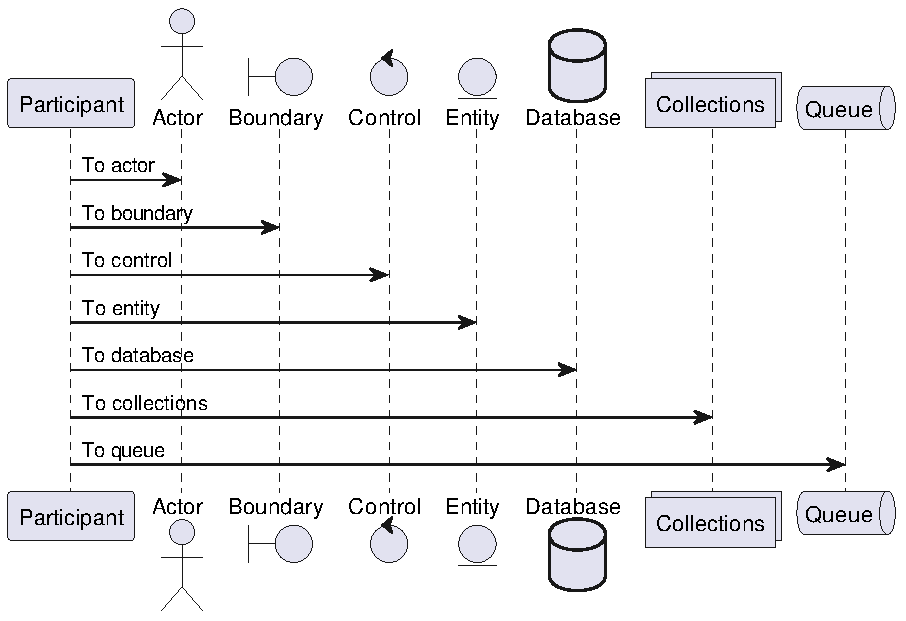
\includegraphics[width=0.8\textwidth]{plantuml/sequence.pdf}
    \caption{graphviz画DFA}
    \label{fig:plantuml_pdf}
\end{figure}
\section{插入graphviz绘图}
\par graphviz\footnote{\url{https://graphviz.org/}}可以绘制更多类型的图表,plantuml就是基于graphviz实现的,建议参考graphviz的画廊\url{https://www.graphviz.org/gallery/},环境配置与操作详见README.md。
\subsection{方案一:导出xdot格式后用dot2tex生成tex后插入}
\par dot2tex稳定性较差,涉及中文等编码问题的情况下可能在WSL中会支持而Windows中不支持。
\begin{figure}[htbp]
    \centering
    \resizebox{0.8\textwidth}{!}{
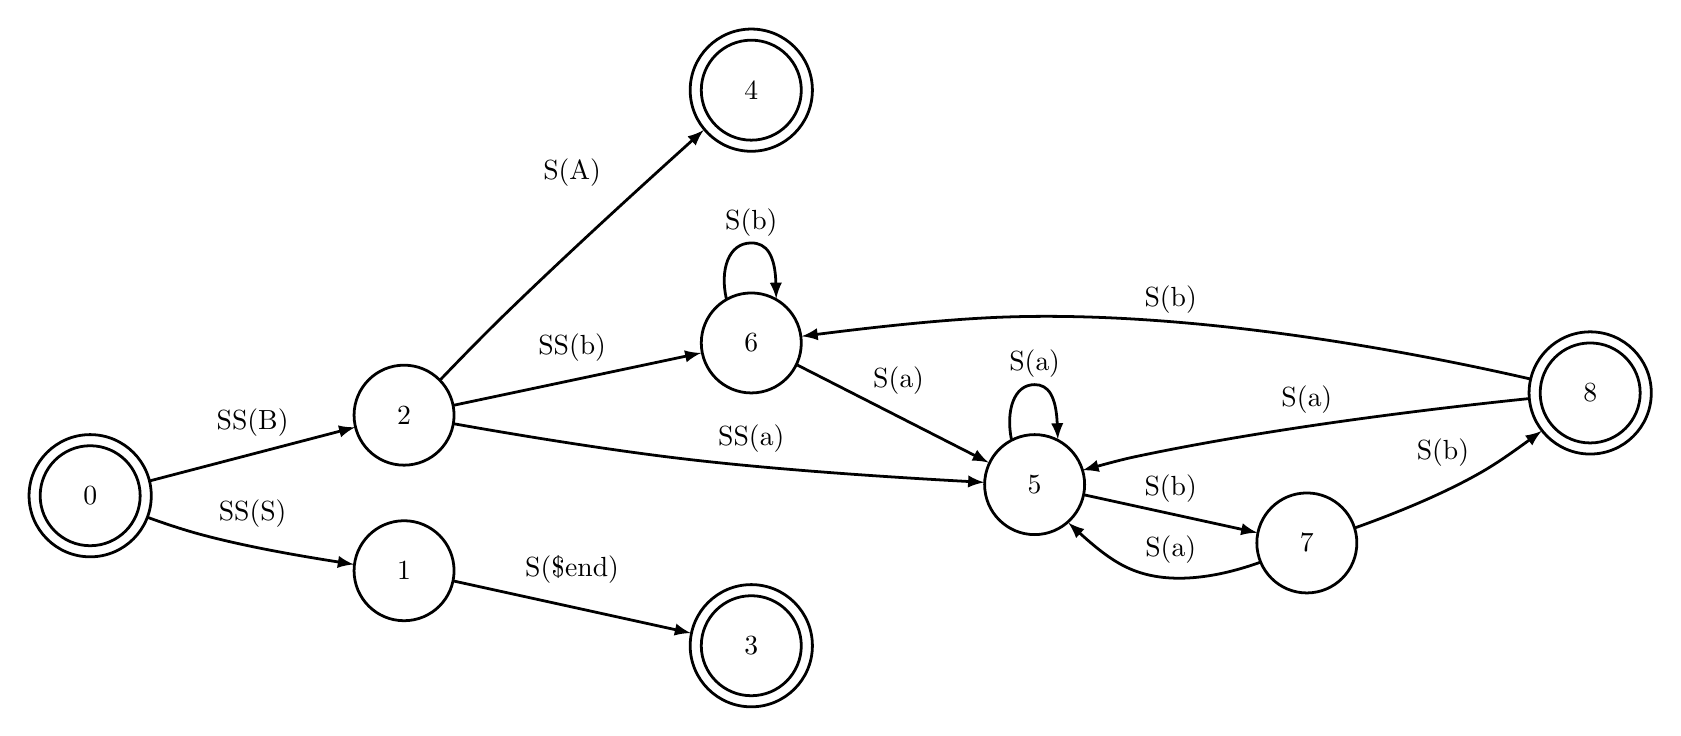
\begin{tikzpicture}[>=latex,line join=bevel,]
  \pgfsetlinewidth{1bp}
%%
\pgfsetcolor{black}
  % Edge: 0 -> 2
  \draw [->] (43.359bp,81.319bp) .. controls (61.397bp,86.032bp) and (87.848bp,92.942bp)  .. (117.39bp,100.66bp);
  \definecolor{strokecol}{rgb}{0.0,0.0,0.0};
  \pgfsetstrokecolor{strokecol}
  \draw (80.5bp,102.5bp) node {SS(B)};
  % Edge: 0 -> 1
  \draw [->] (42.638bp,68.232bp) .. controls (48.772bp,66.002bp) and (55.607bp,63.712bp)  .. (62.0bp,62.0bp) .. controls (76.619bp,58.085bp) and (93.227bp,54.999bp)  .. (116.95bp,51.263bp);
  \draw (80.5bp,69.5bp) node {SS(S)};
  % Edge: 8 -> 6
  \draw [->] (540.44bp,118.03bp) .. controls (502.01bp,126.87bp) and (416.6bp,143.92bp)  .. (344.0bp,140.0bp) .. controls (325.42bp,139.0bp) and (304.6bp,136.74bp)  .. (278.12bp,133.4bp);
  \draw (411.0bp,146.5bp) node {S(b)};
  % Edge: 8 -> 5
  \draw [->] (540.0bp,110.97bp) .. controls (508.8bp,107.75bp) and (448.46bp,100.72bp)  .. (398.0bp,90.0bp) .. controls (395.1bp,89.385bp) and (392.09bp,88.659bp)  .. (379.26bp,85.152bp);
  \draw (460.0bp,110.5bp) node {S(a)};
  % Edge: 2 -> 4
  \draw [->] (148.14bp,117.83bp) .. controls (154.8bp,124.78bp) and (163.25bp,133.46bp)  .. (171.0bp,141.0bp) .. controls (192.29bp,161.72bp) and (217.28bp,184.58bp)  .. (242.85bp,207.63bp);
  \draw (195.5bp,192.5bp) node {S(A)};
  % Edge: 2 -> 6
  \draw [->] (152.84bp,108.56bp) .. controls (173.25bp,112.87bp) and (207.88bp,120.19bp)  .. (241.96bp,127.4bp);
  \draw (195.5bp,129.5bp) node {SS(b)};
  % Edge: 2 -> 5
  \draw [->] (152.91bp,101.91bp) .. controls (173.09bp,98.322bp) and (207.9bp,92.455bp)  .. (238.0bp,89.0bp) .. controls (270.8bp,85.234bp) and (308.71bp,82.74bp)  .. (343.85bp,80.807bp);
  \draw (260.0bp,96.5bp) node {SS(a)};
  % Edge: 1 -> 3
  \draw [->] (152.84bp,45.302bp) .. controls (172.22bp,41.05bp) and (204.41bp,33.982bp)  .. (238.26bp,26.553bp);
  \draw (195.5bp,49.5bp) node {S(\$end)};
  % Edge: 6 -> 6
  \draw [->] (251.02bp,146.92bp) .. controls (248.68bp,157.15bp) and (251.67bp,167.0bp)  .. (260.0bp,167.0bp) .. controls (265.47bp,167.0bp) and (268.63bp,162.76bp)  .. (268.98bp,146.92bp);
  \draw (260.0bp,174.5bp) node {S(b)};
  % Edge: 6 -> 5
  \draw [->] (276.62bp,123.03bp) .. controls (292.62bp,114.87bp) and (317.72bp,102.07bp)  .. (345.48bp,87.913bp);
  \draw (313.0bp,117.5bp) node {S(a)};
  % Edge: 5 -> 5
  \draw [->] (353.64bp,96.29bp) .. controls (351.62bp,106.39bp) and (354.41bp,116.0bp)  .. (362.0bp,116.0bp) .. controls (366.86bp,116.0bp) and (369.76bp,112.06bp)  .. (370.36bp,96.29bp);
  \draw (362.0bp,123.5bp) node {S(a)};
  % Edge: 5 -> 7
  \draw [->] (379.72bp,76.342bp) .. controls (394.22bp,73.17bp) and (415.47bp,68.521bp)  .. (442.15bp,62.686bp);
  \draw (411.0bp,78.5bp) node {S(b)};
  % Edge: 7 -> 8
  \draw [->] (477.31bp,64.421bp) .. controls (489.9bp,68.902bp) and (507.55bp,75.838bp)  .. (522.0bp,84.0bp) .. controls (526.87bp,86.749bp) and (531.83bp,90.018bp)  .. (544.54bp,99.329bp);
  \draw (509.0bp,91.5bp) node {S(b)};
  % Edge: 7 -> 5
  \draw [->] (443.26bp,52.063bp) .. controls (430.67bp,47.534bp) and (412.75bp,43.407bp)  .. (398.0bp,49.0bp) .. controls (392.07bp,51.249bp) and (386.5bp,55.015bp)  .. (374.12bp,66.297bp);
  \draw (411.0bp,56.5bp) node {S(a)};
  % Node: 0
\begin{scope}
  \definecolor{strokecol}{rgb}{0.0,0.0,0.0};
  \pgfsetstrokecolor{strokecol}
  \draw (22.0bp,76.0bp) ellipse (18.0bp and 18.0bp);
  \draw (22.0bp,76.0bp) ellipse (22.0bp and 22.0bp);
  \draw (22.0bp,76.0bp) node {0};
\end{scope}
  % Node: 2
\begin{scope}
  \definecolor{strokecol}{rgb}{0.0,0.0,0.0};
  \pgfsetstrokecolor{strokecol}
  \draw (135.0bp,105.0bp) ellipse (18.0bp and 18.0bp);
  \draw (135.0bp,105.0bp) node {2};
\end{scope}
  % Node: 1
\begin{scope}
  \definecolor{strokecol}{rgb}{0.0,0.0,0.0};
  \pgfsetstrokecolor{strokecol}
  \draw (135.0bp,49.0bp) ellipse (18.0bp and 18.0bp);
  \draw (135.0bp,49.0bp) node {1};
\end{scope}
  % Node: 3
\begin{scope}
  \definecolor{strokecol}{rgb}{0.0,0.0,0.0};
  \pgfsetstrokecolor{strokecol}
  \draw (260.0bp,22.0bp) ellipse (18.0bp and 18.0bp);
  \draw (260.0bp,22.0bp) ellipse (22.0bp and 22.0bp);
  \draw (260.0bp,22.0bp) node {3};
\end{scope}
  % Node: 4
\begin{scope}
  \definecolor{strokecol}{rgb}{0.0,0.0,0.0};
  \pgfsetstrokecolor{strokecol}
  \draw (260.0bp,222.0bp) ellipse (18.0bp and 18.0bp);
  \draw (260.0bp,222.0bp) ellipse (22.0bp and 22.0bp);
  \draw (260.0bp,222.0bp) node {4};
\end{scope}
  % Node: 8
\begin{scope}
  \definecolor{strokecol}{rgb}{0.0,0.0,0.0};
  \pgfsetstrokecolor{strokecol}
  \draw (562.0bp,113.0bp) ellipse (18.0bp and 18.0bp);
  \draw (562.0bp,113.0bp) ellipse (22.0bp and 22.0bp);
  \draw (562.0bp,113.0bp) node {8};
\end{scope}
  % Node: 6
\begin{scope}
  \definecolor{strokecol}{rgb}{0.0,0.0,0.0};
  \pgfsetstrokecolor{strokecol}
  \draw (260.0bp,131.0bp) ellipse (18.0bp and 18.0bp);
  \draw (260.0bp,131.0bp) node {6};
\end{scope}
  % Node: 5
\begin{scope}
  \definecolor{strokecol}{rgb}{0.0,0.0,0.0};
  \pgfsetstrokecolor{strokecol}
  \draw (362.0bp,80.0bp) ellipse (18.0bp and 18.0bp);
  \draw (362.0bp,80.0bp) node {5};
\end{scope}
  % Node: 7
\begin{scope}
  \definecolor{strokecol}{rgb}{0.0,0.0,0.0};
  \pgfsetstrokecolor{strokecol}
  \draw (460.0bp,59.0bp) ellipse (18.0bp and 18.0bp);
  \draw (460.0bp,59.0bp) node {7};
\end{scope}
%
\end{tikzpicture}
}
    \caption{graphviz画DFA}
    \label{fig:graphviz_tex}
\end{figure}
\subsection{方案二:直接导出pdf插入(推荐)}
\par graphviz可以直接导出PDF。如果嵌入plantuml内部,此时plantuml导出PDF不再需要相关依赖jar包,但是不能导出tex。
\begin{figure}[htbp]
    \centering
    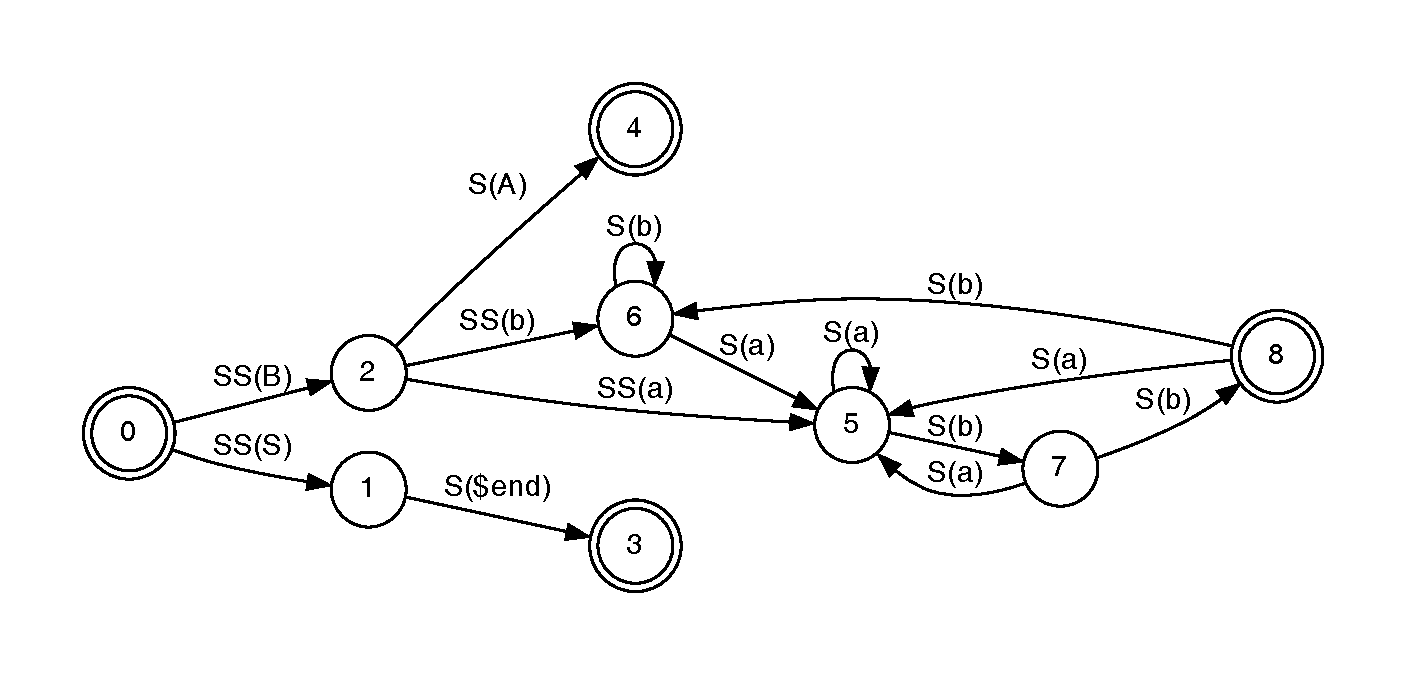
\includegraphics[width=0.8\textwidth]{graphviz/dfa.pdf}
    \caption{graphviz画DFA}
    \label{fig:graphviz_pdf}
\end{figure}
\section{插入svg}
\subsection{方案一:inkscape}
\par inkscape几乎兼容大部分svg图表,但是深层文字可能不会识别被转为图片。
\begin{figure}[htbp]
    \centering
    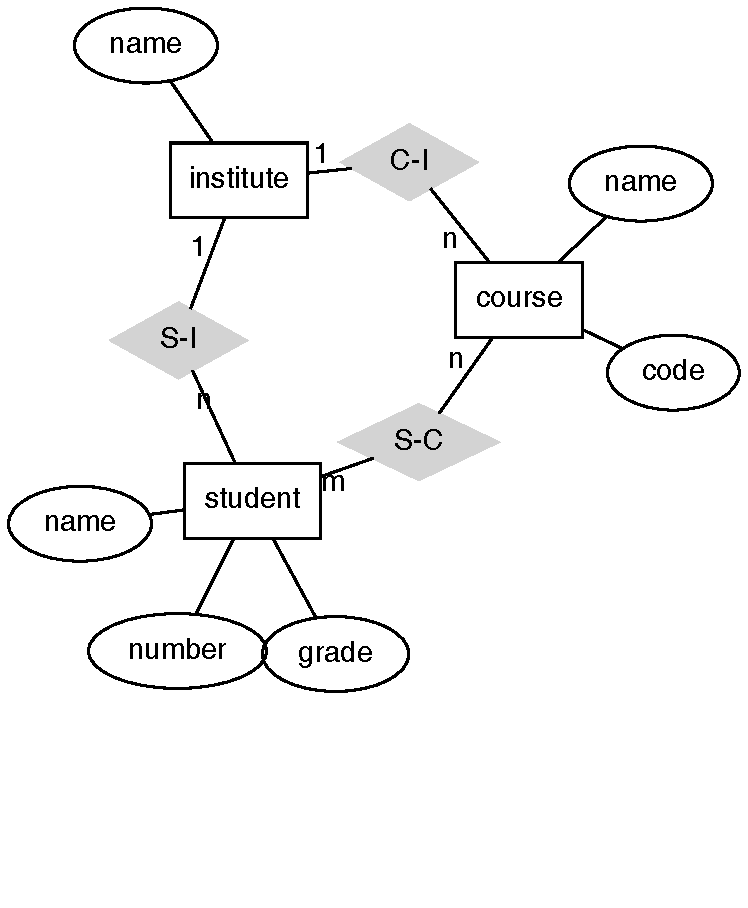
\includegraphics[width=0.8\textwidth]{svg/er_inkscape.pdf}
    \caption{inkscape转svgER图为pdf}
    \label{fig:svg_pdf}
\end{figure}
\begin{figure}[htbp]
    \centering
    \resizebox{0.8\textwidth}{!}{%LaTeX with PSTricks extensions
%%Creator: Inkscape 1.2.2 (732a01da63, 2022-12-09)
%%Please note this file requires PSTricks extensions
\psset{xunit=.5pt,yunit=.5pt,runit=.5pt}
\begin{pspicture}(478.66666667,581.33333333)
{
\newrgbcolor{curcolor}{0 0 0}
\pscustom[linewidth=1.33207173,linecolor=curcolor]
{
\newpath
\moveto(373.02004736,413.31718164)
\lineto(291.76367165,413.31718164)
\lineto(291.76367165,365.36259926)
\lineto(373.02004736,365.36259926)
\closepath
}
}
{
\newrgbcolor{curcolor}{0 0 0}
\pscustom[linestyle=none,fillstyle=solid,fillcolor=curcolor]
{
\newpath
\moveto(313.3012146,387.91701605)
\lineto(313.3012146,387.91701605)
\curveto(313.1312367,386.69074689)(312.69718598,385.75586842)(311.99906245,385.11238064)
\curveto(311.30093892,384.46889286)(310.37213109,384.14714897)(309.21263896,384.14714897)
\curveto(307.91959277,384.14714897)(306.88758407,384.61155289)(306.11661286,385.54036072)
\curveto(305.34564166,386.46916855)(304.96015606,387.71972027)(304.96015606,389.29201587)
\curveto(304.96015606,390.86431148)(305.35778294,392.1148632)(306.1530367,393.04367103)
\curveto(306.9543611,393.9785495)(308.02886428,394.44598873)(309.37654623,394.44598873)
\curveto(310.54817963,394.44598873)(311.4830581,394.12424484)(312.18118163,393.48075706)
\curveto(312.87930516,392.84333993)(313.25264949,391.96309721)(313.3012146,390.84002892)
\lineto(313.3012146,390.84002892)
\lineto(311.72588368,390.84002892)
\lineto(311.72588368,390.84002892)
\curveto(311.65910664,391.53815245)(311.41628107,392.07843936)(310.99740695,392.46088964)
\curveto(310.57853283,392.84333993)(310.020034,393.03456507)(309.32191047,393.03456507)
\curveto(308.49630351,393.03456507)(307.8467451,392.7006799)(307.37323522,392.03290957)
\curveto(306.90579599,391.37120987)(306.67207637,390.45757864)(306.67207637,389.29201587)
\curveto(306.67207637,388.05360543)(306.89061939,387.12176228)(307.32770543,386.49648643)
\curveto(307.76479146,385.87121057)(308.41434988,385.55857264)(309.27638068,385.55857264)
\curveto(309.91379781,385.55857264)(310.44497876,385.76193906)(310.86992352,386.1686719)
\curveto(311.30093892,386.58147538)(311.58625897,387.16425676)(311.72588368,387.91701605)
\lineto(311.72588368,387.91701605)
\closepath
}
}
{
\newrgbcolor{curcolor}{0 0 0}
\pscustom[linestyle=none,fillstyle=solid,fillcolor=curcolor]
{
\newpath
\moveto(318.91048542,384.14714897)
\curveto(317.56280347,384.14714897)(316.47008837,384.62065885)(315.63234014,385.5676786)
\curveto(314.80066254,386.51469834)(314.38482374,387.7561441)(314.38482374,389.29201587)
\curveto(314.38482374,390.83395828)(314.80066254,392.07843936)(315.63234014,393.02545911)
\curveto(316.47008837,393.97247886)(317.56280347,394.44598873)(318.91048542,394.44598873)
\curveto(320.27030864,394.44598873)(321.36605906,393.97247886)(322.19773665,393.02545911)
\curveto(323.02941425,392.07843936)(323.44525305,390.83395828)(323.44525305,389.29201587)
\curveto(323.44525305,387.7561441)(323.02941425,386.51469834)(322.19773665,385.5676786)
\curveto(321.36605906,384.62065885)(320.27030864,384.14714897)(318.91048542,384.14714897)
\closepath
\moveto(318.91048542,385.55857264)
\curveto(319.77251621,385.55857264)(320.45849846,385.89549312)(320.96843217,386.5693341)
\curveto(321.47836589,387.24317507)(321.73333274,388.15073566)(321.73333274,389.29201587)
\curveto(321.73333274,390.43329608)(321.47836589,391.34085667)(320.96843217,392.01469765)
\curveto(320.45849846,392.69460926)(319.77251621,393.03456507)(318.91048542,393.03456507)
\curveto(318.04845462,393.03456507)(317.36247237,392.69460926)(316.85253866,392.01469765)
\curveto(316.34867559,391.34085667)(316.09674405,390.43329608)(316.09674405,389.29201587)
\curveto(316.09674405,388.15073566)(316.34867559,387.24317507)(316.85253866,386.5693341)
\curveto(317.36247237,385.89549312)(318.04845462,385.55857264)(318.91048542,385.55857264)
\closepath
}
}
{
\newrgbcolor{curcolor}{0 0 0}
\pscustom[linestyle=none,fillstyle=solid,fillcolor=curcolor]
{
\newpath
\moveto(327.00568307,394.15459804)
\lineto(327.00568307,387.87148625)
\curveto(327.00568307,387.05194993)(327.16351969,386.46006259)(327.47919294,386.09582422)
\curveto(327.79486619,385.7376565)(328.30783522,385.55857264)(329.01810003,385.55857264)
\curveto(329.80728315,385.55857264)(330.43255901,385.86210461)(330.89392761,386.46916855)
\curveto(331.3552962,387.08230313)(331.5859805,387.91094541)(331.5859805,388.95509539)
\lineto(331.5859805,388.95509539)
\lineto(331.5859805,394.15459804)
\lineto(331.5859805,394.15459804)
\lineto(332.40551682,394.15459804)
\lineto(333.22505314,394.15459804)
\lineto(333.22505314,394.15459804)
\lineto(333.22505314,384.41122179)
\lineto(333.22505314,384.41122179)
\lineto(332.45104661,384.41122179)
\lineto(331.66793413,384.41122179)
\lineto(331.66793413,384.41122179)
\lineto(331.66793413,385.89549312)
\lineto(331.66793413,385.89549312)
\lineto(331.66793413,385.89549312)
\curveto(331.55866262,385.71944458)(331.43724983,385.552502)(331.30369577,385.39466537)
\curveto(330.60557223,384.56298777)(329.73140016,384.14714897)(328.68117954,384.14714897)
\curveto(327.57632317,384.14714897)(326.74768089,384.42336307)(326.1952527,384.97579125)
\curveto(325.64282452,385.52821944)(325.36661043,386.35686172)(325.36661043,387.46171809)
\lineto(325.36661043,394.15459804)
\lineto(325.36661043,394.15459804)
\lineto(326.18614675,394.15459804)
\lineto(327.00568307,394.15459804)
\closepath
}
}
{
\newrgbcolor{curcolor}{0 0 0}
\pscustom[linestyle=none,fillstyle=solid,fillcolor=curcolor]
{
\newpath
\moveto(335.91131108,384.41122179)
\lineto(335.91131108,394.15459804)
\lineto(335.91131108,394.15459804)
\lineto(336.6853176,394.15459804)
\lineto(337.46843008,394.15459804)
\lineto(337.46843008,394.15459804)
\lineto(337.46843008,392.48820752)
\lineto(337.46843008,392.48820752)
\lineto(337.46843008,392.48820752)
\curveto(337.60805479,392.74924502)(337.75678546,392.98599995)(337.91462208,393.19847233)
\curveto(338.5338273,394.03014993)(339.29569255,394.44598873)(340.20021782,394.44598873)
\curveto(340.3519838,394.44598873)(340.50678511,394.41867085)(340.66462173,394.3640351)
\lineto(340.66462173,392.68853862)
\lineto(340.32770125,392.69764458)
\curveto(339.44138789,392.69764458)(338.75540564,392.43053645)(338.26975449,391.89632018)
\curveto(337.79017397,391.36817455)(337.55038372,390.61237994)(337.55038372,389.62893636)
\lineto(337.55038372,389.62893636)
\lineto(337.55038372,384.41122179)
\lineto(337.55038372,384.41122179)
\lineto(336.7308474,384.41122179)
\lineto(335.91131108,384.41122179)
\closepath
}
}
{
\newrgbcolor{curcolor}{0 0 0}
\pscustom[linestyle=none,fillstyle=solid,fillcolor=curcolor]
{
\newpath
\moveto(347.47587915,391.33175071)
\lineto(347.47587915,391.33175071)
\curveto(347.42731403,391.87203762)(347.20573569,392.29091174)(346.81114413,392.58837307)
\curveto(346.42262321,392.8858344)(345.8975129,393.03456507)(345.23581321,393.03456507)
\curveto(344.55590159,393.03456507)(344.03686192,392.9161876)(343.6786942,392.67943266)
\curveto(343.32659711,392.44267773)(343.15054857,392.09665128)(343.15054857,391.64135332)
\curveto(343.15054857,391.29532688)(343.27499668,391.03428938)(343.52389289,390.85824084)
\curveto(343.77278911,390.6821923)(344.26754622,390.50614375)(345.00816423,390.33009521)
\lineto(346.70187262,389.92943301)
\curveto(347.64889237,389.69874871)(348.32576867,389.38004014)(348.73250151,388.9733073)
\curveto(349.13316371,388.5726451)(349.33349481,388.01111096)(349.33349481,387.28870487)
\curveto(349.33349481,386.3234732)(348.98443304,385.55857264)(348.28630951,384.99400317)
\curveto(347.59425662,384.42943371)(346.65634283,384.14714897)(345.47256814,384.14714897)
\curveto(344.10060364,384.14714897)(343.0777009,384.41729243)(342.40385992,384.95757934)
\curveto(341.73001895,385.50393688)(341.35667463,386.35989704)(341.28382695,387.5254598)
\lineto(341.28382695,387.5254598)
\lineto(342.85915788,387.5254598)
\lineto(342.85915788,387.5254598)
\curveto(342.93807619,386.83340691)(343.18090177,386.33257916)(343.58763461,386.02297655)
\curveto(344.00043809,385.71337394)(344.62874927,385.55857264)(345.47256814,385.55857264)
\curveto(346.20711551,385.55857264)(346.76257902,385.69819734)(347.13895866,385.97744676)
\curveto(347.52140894,386.25669617)(347.71263409,386.66342901)(347.71263409,387.19764528)
\curveto(347.71263409,387.53760108)(347.58818598,387.79560326)(347.33928976,387.9716518)
\curveto(347.09039355,388.14770034)(346.58956579,388.32374889)(345.83680651,388.49979743)
\lineto(344.14309811,388.90045963)
\curveto(343.22643156,389.11900265)(342.57383783,389.42556994)(342.1853169,389.8201615)
\curveto(341.79679598,390.20868242)(341.60253552,390.75503997)(341.60253552,391.45923414)
\curveto(341.60253552,392.37590069)(341.92731473,393.1013421)(342.57687315,393.63555837)
\curveto(343.2325022,394.17584528)(344.11881556,394.44598873)(345.23581321,394.44598873)
\curveto(346.37102278,394.44598873)(347.27251273,394.16977464)(347.94028306,393.61734645)
\curveto(348.61412404,393.06491826)(348.97229176,392.30305302)(349.01478624,391.33175071)
\lineto(349.01478624,391.33175071)
\closepath
}
}
{
\newrgbcolor{curcolor}{0 0 0}
\pscustom[linestyle=none,fillstyle=solid,fillcolor=curcolor]
{
\newpath
\moveto(355.18862652,384.14714897)
\curveto(353.81059137,384.14714897)(352.72698224,384.58423501)(351.93779911,385.45840709)
\curveto(351.14861599,386.33257916)(350.75402443,387.5406364)(350.75402443,389.08257881)
\curveto(350.75402443,390.72165145)(351.16986323,392.02380361)(352.00154083,392.98903527)
\curveto(352.83928907,393.96033758)(353.96235736,394.44598873)(355.3707457,394.44598873)
\curveto(356.64557997,394.44598873)(357.67455335,393.97247886)(358.45766584,393.02545911)
\curveto(359.24077832,392.07843936)(359.63233456,390.83395828)(359.63233456,389.29201587)
\lineto(359.61412264,388.70923449)
\lineto(359.61412264,388.70923449)
\lineto(352.49326262,388.70923449)
\lineto(352.49326262,388.70923449)
\curveto(352.56003965,387.73793218)(352.78161799,386.99731418)(353.15799763,386.48738047)
\curveto(353.61936623,385.86817525)(354.34784296,385.55857264)(355.34342782,385.55857264)
\curveto(355.96870368,385.55857264)(356.51506123,385.73462118)(356.98250046,386.08671827)
\curveto(357.4499397,386.43881535)(357.73525975,386.88804267)(357.83846062,387.43440021)
\lineto(357.83846062,387.43440021)
\lineto(359.45932134,387.43440021)
\lineto(359.45932134,387.43440021)
\curveto(359.21649576,386.36596768)(358.73084461,385.54946668)(358.00236788,384.98489721)
\curveto(357.27389115,384.42639839)(356.33597736,384.14714897)(355.18862652,384.14714897)
\closepath
\moveto(357.92041425,390.02959856)
\lineto(357.92041425,390.02959856)
\curveto(357.87184913,390.93412383)(357.64723548,391.638318)(357.24657328,392.14218107)
\curveto(356.8034166,392.7006799)(356.15385818,392.97992931)(355.29789803,392.97992931)
\curveto(354.43586723,392.97992931)(353.74684966,392.65818542)(353.23084531,392.01469765)
\curveto(352.82411247,391.51083458)(352.57825157,390.84913488)(352.49326262,390.02959856)
\lineto(352.49326262,390.02959856)
\closepath
}
}
{
\newrgbcolor{curcolor}{0.82745099 0.82745099 0.82745099}
\pscustom[linestyle=none,fillstyle=solid,fillcolor=curcolor]
{
\newpath
\moveto(262.03183058,501.23391601)
\lineto(218.95263073,477.25662482)
\lineto(262.03183058,453.27933363)
\lineto(305.11103042,477.25662482)
\closepath
}
}
{
\newrgbcolor{curcolor}{0.82745099 0.82745099 0.82745099}
\pscustom[linewidth=1.33207173,linecolor=curcolor]
{
\newpath
\moveto(262.03183058,501.23391601)
\lineto(218.95263073,477.25662482)
\lineto(262.03183058,453.27933363)
\lineto(305.11103042,477.25662482)
\closepath
}
}
{
\newrgbcolor{curcolor}{0 0 0}
\pscustom[linestyle=none,fillstyle=solid,fillcolor=curcolor]
{
\newpath
\moveto(262.30501829,477.25428004)
\lineto(262.30501829,477.25428004)
\curveto(262.07433399,475.60306612)(261.43995218,474.30698461)(260.40187284,473.3660355)
\curveto(259.36986414,472.43115703)(258.06164135,471.96371779)(256.47720446,471.96371779)
\curveto(254.63173008,471.96371779)(253.15960002,472.59809961)(252.06081429,473.86686325)
\curveto(250.9680992,475.14169752)(250.42174165,476.85665316)(250.42174165,479.01173015)
\curveto(250.42174165,481.16680714)(250.98934644,482.88176277)(252.12455601,484.15659704)
\curveto(253.26583621,485.43750196)(254.79563734,486.07795442)(256.7139594,486.07795442)
\curveto(258.22554861,486.07795442)(259.46699437,485.6894335)(260.43829667,484.91239165)
\curveto(261.40959898,484.13534981)(261.99238036,483.06388195)(262.18664082,481.69798808)
\lineto(262.18664082,481.69798808)
\lineto(260.43829667,481.69798808)
\lineto(260.43829667,481.69798808)
\curveto(260.26831877,482.58430144)(259.85551529,483.26724837)(259.19988624,483.74682888)
\curveto(258.55032782,484.23248004)(257.71257958,484.47530561)(256.68664152,484.47530561)
\curveto(255.34503021,484.47530561)(254.27659768,483.9805485)(253.48134391,482.99103428)
\curveto(252.68609015,482.00759069)(252.28846327,480.68115598)(252.28846327,479.01173015)
\curveto(252.28846327,477.23910344)(252.65573695,475.88838617)(253.39028432,474.95957834)
\curveto(254.13090233,474.03077051)(255.20237019,473.5663666)(256.60468789,473.5663666)
\curveto(257.64276723,473.5663666)(258.50479802,473.88507517)(259.19078028,474.5224923)
\curveto(259.87676253,475.16598008)(260.33206048,476.07657599)(260.55667414,477.25428004)
\lineto(260.55667414,477.25428004)
\closepath
}
}
{
\newrgbcolor{curcolor}{0 0 0}
\pscustom[linestyle=none,fillstyle=solid,fillcolor=curcolor]
{
\newpath
\moveto(263.88945518,478.32878321)
\lineto(268.46064665,478.32878321)
\lineto(268.46064665,476.64418078)
\lineto(263.88945518,476.64418078)
\closepath
}
}
{
\newrgbcolor{curcolor}{0 0 0}
\pscustom[linestyle=none,fillstyle=solid,fillcolor=curcolor]
{
\newpath
\moveto(270.97389137,472.32795616)
\lineto(270.97389137,485.71371605)
\lineto(270.97389137,485.71371605)
\lineto(271.87538132,485.71371605)
\lineto(272.78597723,485.71371605)
\lineto(272.78597723,485.71371605)
\lineto(272.78597723,472.32795616)
\lineto(272.78597723,472.32795616)
\lineto(271.88448728,472.32795616)
\lineto(270.97389137,472.32795616)
\closepath
}
}
{
\newrgbcolor{curcolor}{0 0 0}
\pscustom[linewidth=1.33207173,linecolor=curcolor]
{
\newpath
\moveto(312.79708432,413.8233689)
\curveto(300.91500446,428.66264801)(286.07572535,447.20508653)(275.51239651,460.4059174)
}
}
{
\newrgbcolor{curcolor}{0 0 0}
\pscustom[linestyle=none,fillstyle=solid,fillcolor=curcolor]
{
\newpath
\moveto(284.19232926,422.20209035)
\lineto(284.19232926,431.9454666)
\lineto(284.19232926,431.9454666)
\lineto(284.96633579,431.9454666)
\lineto(285.74944827,431.9454666)
\lineto(285.74944827,431.9454666)
\lineto(285.74944827,430.50672506)
\lineto(285.74944827,430.50672506)
\lineto(285.74944827,430.50672506)
\lineto(286.11368663,430.98934089)
\curveto(286.82395144,431.82101849)(287.71330012,432.23685729)(288.78173265,432.23685729)
\curveto(289.85623583,432.23685729)(290.68487811,431.9454666)(291.26765949,431.36268521)
\curveto(291.85044087,430.77990383)(292.14183157,429.95126155)(292.14183157,428.87675838)
\lineto(292.14183157,422.20209035)
\lineto(292.14183157,422.20209035)
\lineto(291.32229525,422.20209035)
\lineto(290.50275893,422.20209035)
\lineto(290.50275893,422.20209035)
\lineto(290.50275893,428.32129487)
\curveto(290.50275893,429.17725503)(290.33581634,429.79342493)(290.00193117,430.16980457)
\curveto(289.67411665,430.55225485)(289.13990038,430.74347999)(288.39928237,430.74347999)
\curveto(287.61009925,430.74347999)(286.98482339,430.44298334)(286.52345479,429.84199004)
\curveto(286.0620862,429.24706738)(285.8314019,428.43967234)(285.8314019,427.41980492)
\lineto(285.8314019,427.41980492)
\lineto(285.8314019,422.20209035)
\lineto(285.8314019,422.20209035)
\lineto(285.01186558,422.20209035)
\lineto(284.19232926,422.20209035)
\closepath
}
}
{
\newrgbcolor{curcolor}{0 0 0}
\pscustom[linewidth=1.33207173,linecolor=curcolor]
{
\newpath
\moveto(196.80027782,489.59160907)
\lineto(108.88354345,489.59160907)
\lineto(108.88354345,441.63702669)
\lineto(196.80027782,441.63702669)
\closepath
}
}
{
\newrgbcolor{curcolor}{0 0 0}
\pscustom[linestyle=none,fillstyle=solid,fillcolor=curcolor]
{
\newpath
\moveto(121.9727064,460.68566222)
\lineto(121.9727064,470.42903847)
\lineto(121.9727064,470.42903847)
\lineto(122.79224272,470.42903847)
\lineto(123.61177904,470.42903847)
\lineto(123.61177904,470.42903847)
\lineto(123.61177904,460.68566222)
\lineto(123.61177904,460.68566222)
\lineto(122.79224272,460.68566222)
\lineto(121.9727064,460.68566222)
\closepath
\moveto(121.95449448,474.07142212)
\lineto(123.62999096,474.07142212)
\lineto(123.62999096,472.21380646)
\lineto(121.95449448,472.21380646)
\closepath
}
}
{
\newrgbcolor{curcolor}{0 0 0}
\pscustom[linestyle=none,fillstyle=solid,fillcolor=curcolor]
{
\newpath
\moveto(126.06128204,460.68566222)
\lineto(126.06128204,470.42903847)
\lineto(126.06128204,470.42903847)
\lineto(126.83528856,470.42903847)
\lineto(127.61840105,470.42903847)
\lineto(127.61840105,470.42903847)
\lineto(127.61840105,468.99029693)
\lineto(127.61840105,468.99029693)
\lineto(127.61840105,468.99029693)
\lineto(127.98263941,469.47291276)
\curveto(128.69290422,470.30459036)(129.58225289,470.72042916)(130.65068543,470.72042916)
\curveto(131.72518861,470.72042916)(132.55383088,470.42903847)(133.13661227,469.84625709)
\curveto(133.71939365,469.26347571)(134.01078434,468.43483343)(134.01078434,467.36033025)
\lineto(134.01078434,460.68566222)
\lineto(134.01078434,460.68566222)
\lineto(133.19124802,460.68566222)
\lineto(132.3717117,460.68566222)
\lineto(132.3717117,460.68566222)
\lineto(132.3717117,466.80486675)
\curveto(132.3717117,467.6608269)(132.20476912,468.2769968)(131.87088395,468.65337644)
\curveto(131.54306942,469.03582673)(131.00885316,469.22705187)(130.26823515,469.22705187)
\curveto(129.47905202,469.22705187)(128.85377617,468.92655522)(128.39240757,468.32556192)
\curveto(127.93103898,467.73063925)(127.70035468,466.92324421)(127.70035468,465.90337679)
\lineto(127.70035468,465.90337679)
\lineto(127.70035468,460.68566222)
\lineto(127.70035468,460.68566222)
\lineto(126.88081836,460.68566222)
\lineto(126.06128204,460.68566222)
\closepath
}
}
{
\newrgbcolor{curcolor}{0 0 0}
\pscustom[linestyle=none,fillstyle=solid,fillcolor=curcolor]
{
\newpath
\moveto(142.0149224,467.60619115)
\lineto(142.0149224,467.60619115)
\curveto(141.96635729,468.14647805)(141.74477895,468.56535217)(141.35018739,468.8628135)
\curveto(140.96166646,469.16027484)(140.43655616,469.3090055)(139.77485646,469.3090055)
\curveto(139.09494485,469.3090055)(138.57590518,469.19062803)(138.21773745,468.9538731)
\curveto(137.86564037,468.71711816)(137.68959182,468.37109171)(137.68959182,467.91579376)
\curveto(137.68959182,467.56976731)(137.81403993,467.30872982)(138.06293615,467.13268127)
\curveto(138.31183236,466.95663273)(138.80658947,466.78058419)(139.54720748,466.60453564)
\lineto(141.24091588,466.20387344)
\curveto(142.18793562,465.97318915)(142.86481192,465.65448058)(143.27154476,465.24774774)
\curveto(143.67220696,464.84708554)(143.87253806,464.28555139)(143.87253806,463.5631453)
\curveto(143.87253806,462.59791364)(143.52347629,461.83301307)(142.82535276,461.26844361)
\curveto(142.13329987,460.70387414)(141.19538608,460.42158941)(140.0116114,460.42158941)
\curveto(138.63964689,460.42158941)(137.61674415,460.69173286)(136.94290318,461.23201977)
\curveto(136.2690622,461.77837732)(135.89571788,462.63433747)(135.82287021,463.79990024)
\lineto(135.82287021,463.79990024)
\lineto(137.39820113,463.79990024)
\lineto(137.39820113,463.79990024)
\curveto(137.47711944,463.10784735)(137.71994502,462.60701959)(138.12667786,462.29741698)
\curveto(138.53948134,461.98781438)(139.16779252,461.83301307)(140.0116114,461.83301307)
\curveto(140.74615877,461.83301307)(141.30162227,461.97263778)(141.67800191,462.25188719)
\curveto(142.0604522,462.5311366)(142.25167734,462.93786944)(142.25167734,463.47208571)
\curveto(142.25167734,463.81204152)(142.12722923,464.07004369)(141.87833302,464.24609223)
\curveto(141.6294368,464.42214078)(141.12860905,464.59818932)(140.37584976,464.77423786)
\lineto(138.68214137,465.17490006)
\curveto(137.76547482,465.39344308)(137.11288108,465.70001037)(136.72436016,466.09460193)
\curveto(136.33583924,466.48312286)(136.14157877,467.0294804)(136.14157877,467.73367457)
\curveto(136.14157877,468.65034112)(136.46635798,469.37578253)(137.1159164,469.9099988)
\curveto(137.77154546,470.45028571)(138.65785881,470.72042916)(139.77485646,470.72042916)
\curveto(140.91006603,470.72042916)(141.81155598,470.44421507)(142.47932632,469.89178688)
\curveto(143.15316729,469.3393587)(143.51133502,468.57749345)(143.55382949,467.60619115)
\lineto(143.55382949,467.60619115)
\closepath
}
}
{
\newrgbcolor{curcolor}{0 0 0}
\pscustom[linestyle=none,fillstyle=solid,fillcolor=curcolor]
{
\newpath
\moveto(149.33611353,460.69476818)
\curveto(148.7776147,460.60977923)(148.37088186,460.56728475)(148.11591501,460.56728475)
\curveto(147.39957956,460.56728475)(146.89268117,460.72512138)(146.59521983,461.04079463)
\curveto(146.30382914,461.35646788)(146.1581338,461.8997901)(146.1581338,462.67076131)
\lineto(146.1581338,469.09046248)
\lineto(146.1581338,469.09046248)
\lineto(144.81045185,469.09046248)
\lineto(144.81045185,470.42903847)
\lineto(146.1581338,470.42903847)
\lineto(146.1581338,470.42903847)
\lineto(146.1581338,473.1608262)
\lineto(147.79720644,473.1608262)
\lineto(147.79720644,470.42903847)
\lineto(147.79720644,470.42903847)
\lineto(149.33611353,470.42903847)
\lineto(149.33611353,469.09046248)
\lineto(147.79720644,469.09046248)
\lineto(147.79720644,469.09046248)
\lineto(147.79720644,462.67076131)
\curveto(147.79720644,462.45221829)(147.88219539,462.27920507)(148.05217329,462.15172164)
\curveto(148.22822184,462.02423821)(148.46194145,461.9604965)(148.75333214,461.9604965)
\lineto(149.33611353,461.9604965)
\closepath
}
}
{
\newrgbcolor{curcolor}{0 0 0}
\pscustom[linestyle=none,fillstyle=solid,fillcolor=curcolor]
{
\newpath
\moveto(150.99339809,460.68566222)
\lineto(150.99339809,470.42903847)
\lineto(150.99339809,470.42903847)
\lineto(151.81293441,470.42903847)
\lineto(152.63247073,470.42903847)
\lineto(152.63247073,470.42903847)
\lineto(152.63247073,460.68566222)
\lineto(152.63247073,460.68566222)
\lineto(151.81293441,460.68566222)
\lineto(150.99339809,460.68566222)
\closepath
\moveto(150.97518617,474.07142212)
\lineto(152.65068264,474.07142212)
\lineto(152.65068264,472.21380646)
\lineto(150.97518617,472.21380646)
\closepath
}
}
{
\newrgbcolor{curcolor}{0 0 0}
\pscustom[linestyle=none,fillstyle=solid,fillcolor=curcolor]
{
\newpath
\moveto(158.66061566,460.69476818)
\curveto(158.10211683,460.60977923)(157.69538399,460.56728475)(157.44041714,460.56728475)
\curveto(156.72408169,460.56728475)(156.2171833,460.72512138)(155.91972197,461.04079463)
\curveto(155.62833127,461.35646788)(155.48263593,461.8997901)(155.48263593,462.67076131)
\lineto(155.48263593,469.09046248)
\lineto(155.48263593,469.09046248)
\lineto(154.13495398,469.09046248)
\lineto(154.13495398,470.42903847)
\lineto(155.48263593,470.42903847)
\lineto(155.48263593,470.42903847)
\lineto(155.48263593,473.1608262)
\lineto(157.12170857,473.1608262)
\lineto(157.12170857,470.42903847)
\lineto(157.12170857,470.42903847)
\lineto(158.66061566,470.42903847)
\lineto(158.66061566,469.09046248)
\lineto(157.12170857,469.09046248)
\lineto(157.12170857,469.09046248)
\lineto(157.12170857,462.67076131)
\curveto(157.12170857,462.45221829)(157.20669752,462.27920507)(157.37667542,462.15172164)
\curveto(157.55272397,462.02423821)(157.78644358,461.9604965)(158.07783427,461.9604965)
\lineto(158.66061566,461.9604965)
\closepath
}
}
{
\newrgbcolor{curcolor}{0 0 0}
\pscustom[linestyle=none,fillstyle=solid,fillcolor=curcolor]
{
\newpath
\moveto(161.95697286,470.42903847)
\lineto(161.95697286,464.14592668)
\curveto(161.95697286,463.32639036)(162.11480948,462.73450302)(162.43048273,462.37026466)
\curveto(162.74615598,462.01209693)(163.25912501,461.83301307)(163.96938982,461.83301307)
\curveto(164.75857294,461.83301307)(165.3838488,462.13654504)(165.8452174,462.74360898)
\curveto(166.30658599,463.35674356)(166.53727029,464.18538584)(166.53727029,465.22953582)
\lineto(166.53727029,465.22953582)
\lineto(166.53727029,470.42903847)
\lineto(166.53727029,470.42903847)
\lineto(167.35680661,470.42903847)
\lineto(168.17634293,470.42903847)
\lineto(168.17634293,470.42903847)
\lineto(168.17634293,460.68566222)
\lineto(168.17634293,460.68566222)
\lineto(167.4023364,460.68566222)
\lineto(166.61922392,460.68566222)
\lineto(166.61922392,460.68566222)
\lineto(166.61922392,462.16993356)
\lineto(166.61922392,462.16993356)
\lineto(166.61922392,462.16993356)
\curveto(166.50995241,461.99388501)(166.38853962,461.82694243)(166.25498556,461.66910581)
\curveto(165.55686202,460.83742821)(164.68268995,460.42158941)(163.63246933,460.42158941)
\curveto(162.52761296,460.42158941)(161.69897068,460.6978035)(161.1465425,461.25023169)
\curveto(160.59411431,461.80265987)(160.31790022,462.63130215)(160.31790022,463.73615852)
\lineto(160.31790022,470.42903847)
\lineto(160.31790022,470.42903847)
\lineto(161.13743654,470.42903847)
\lineto(161.95697286,470.42903847)
\closepath
}
}
{
\newrgbcolor{curcolor}{0 0 0}
\pscustom[linestyle=none,fillstyle=solid,fillcolor=curcolor]
{
\newpath
\moveto(174.21359382,460.69476818)
\curveto(173.65509499,460.60977923)(173.24836215,460.56728475)(172.9933953,460.56728475)
\curveto(172.27705985,460.56728475)(171.77016146,460.72512138)(171.47270013,461.04079463)
\curveto(171.18130944,461.35646788)(171.03561409,461.8997901)(171.03561409,462.67076131)
\lineto(171.03561409,469.09046248)
\lineto(171.03561409,469.09046248)
\lineto(169.68793214,469.09046248)
\lineto(169.68793214,470.42903847)
\lineto(171.03561409,470.42903847)
\lineto(171.03561409,470.42903847)
\lineto(171.03561409,473.1608262)
\lineto(172.67468673,473.1608262)
\lineto(172.67468673,470.42903847)
\lineto(172.67468673,470.42903847)
\lineto(174.21359382,470.42903847)
\lineto(174.21359382,469.09046248)
\lineto(172.67468673,469.09046248)
\lineto(172.67468673,469.09046248)
\lineto(172.67468673,462.67076131)
\curveto(172.67468673,462.45221829)(172.75967568,462.27920507)(172.92965359,462.15172164)
\curveto(173.10570213,462.02423821)(173.33942175,461.9604965)(173.63081244,461.9604965)
\lineto(174.21359382,461.9604965)
\closepath
}
}
{
\newrgbcolor{curcolor}{0 0 0}
\pscustom[linestyle=none,fillstyle=solid,fillcolor=curcolor]
{
\newpath
\moveto(179.7864408,460.42158941)
\curveto(178.40840565,460.42158941)(177.32479652,460.85867545)(176.53561339,461.73284752)
\curveto(175.74643027,462.60701959)(175.35183871,463.81507684)(175.35183871,465.35701925)
\curveto(175.35183871,466.99609189)(175.76767751,468.29824404)(176.59935511,469.26347571)
\curveto(177.43710335,470.23477801)(178.56017164,470.72042916)(179.96855998,470.72042916)
\curveto(181.24339425,470.72042916)(182.27236763,470.24691929)(183.05548012,469.29989954)
\curveto(183.8385926,468.35287979)(184.23014884,467.10839872)(184.23014884,465.56645631)
\lineto(184.21193692,464.98367492)
\lineto(184.21193692,464.98367492)
\lineto(177.0910769,464.98367492)
\lineto(177.0910769,464.98367492)
\curveto(177.15785393,464.01237262)(177.37943227,463.27175461)(177.75581191,462.7618209)
\curveto(178.21718051,462.14261568)(178.94565724,461.83301307)(179.9412421,461.83301307)
\curveto(180.56651796,461.83301307)(181.11287551,462.00906161)(181.58031474,462.3611587)
\curveto(182.04775398,462.71325578)(182.33307403,463.1624831)(182.4362749,463.70884065)
\lineto(182.4362749,463.70884065)
\lineto(184.05713562,463.70884065)
\lineto(184.05713562,463.70884065)
\curveto(183.81431004,462.64040811)(183.32865889,461.82390711)(182.60018216,461.25933765)
\curveto(181.87170543,460.70083882)(180.93379164,460.42158941)(179.7864408,460.42158941)
\closepath
\moveto(182.51822853,466.30403899)
\lineto(182.51822853,466.30403899)
\curveto(182.46966341,467.20856427)(182.24504976,467.91275844)(181.84438756,468.41662151)
\curveto(181.40123088,468.97512033)(180.75167246,469.25436975)(179.89571231,469.25436975)
\curveto(179.03368151,469.25436975)(178.34466394,468.93262586)(177.82865959,468.28913808)
\curveto(177.42192675,467.78527501)(177.17606585,467.12357531)(177.0910769,466.30403899)
\lineto(177.0910769,466.30403899)
\closepath
}
}
{
\newrgbcolor{curcolor}{0 0 0}
\pscustom[linewidth=1.33207173,linecolor=curcolor]
{
\newpath
\moveto(139.20149609,551.99916325)
\curveto(139.20149609,538.75687099)(118.69168461,528.02187206)(93.39155001,528.02187206)
\curveto(68.0914154,528.02187206)(47.58160392,538.75687099)(47.58160392,551.99916325)
\curveto(47.58160392,565.24145551)(68.0914154,575.97645444)(93.39155001,575.97645444)
\curveto(118.69168461,575.97645444)(139.20149609,565.24145551)(139.20149609,551.99916325)
\closepath
}
}
{
\newrgbcolor{curcolor}{0 0 0}
\pscustom[linestyle=none,fillstyle=solid,fillcolor=curcolor]
{
\newpath
\moveto(71.2777283,547.07052223)
\lineto(71.2777283,556.81389848)
\lineto(71.2777283,556.81389848)
\lineto(72.05173483,556.81389848)
\lineto(72.83484731,556.81389848)
\lineto(72.83484731,556.81389848)
\lineto(72.83484731,555.37515694)
\lineto(72.83484731,555.37515694)
\lineto(72.83484731,555.37515694)
\lineto(73.19908568,555.85777277)
\curveto(73.90935049,556.68945037)(74.79869916,557.10528917)(75.8671317,557.10528917)
\curveto(76.94163487,557.10528917)(77.77027715,556.81389848)(78.35305853,556.2311171)
\curveto(78.93583992,555.64833571)(79.22723061,554.81969343)(79.22723061,553.74519026)
\lineto(79.22723061,547.07052223)
\lineto(79.22723061,547.07052223)
\lineto(78.40769429,547.07052223)
\lineto(77.58815797,547.07052223)
\lineto(77.58815797,547.07052223)
\lineto(77.58815797,553.18972675)
\curveto(77.58815797,554.04568691)(77.42121538,554.66185681)(77.08733022,555.03823645)
\curveto(76.75951569,555.42068674)(76.22529942,555.61191188)(75.48468141,555.61191188)
\curveto(74.69549829,555.61191188)(74.07022243,555.31141523)(73.60885384,554.71042192)
\curveto(73.14748524,554.11549926)(72.91680094,553.30810422)(72.91680094,552.2882368)
\lineto(72.91680094,552.2882368)
\lineto(72.91680094,547.07052223)
\lineto(72.91680094,547.07052223)
\lineto(72.09726462,547.07052223)
\lineto(71.2777283,547.07052223)
\closepath
}
}
{
\newrgbcolor{curcolor}{0 0 0}
\pscustom[linestyle=none,fillstyle=solid,fillcolor=curcolor]
{
\newpath
\moveto(84.2172962,546.80644942)
\curveto(83.26420581,546.80644942)(82.50841121,547.06141627)(81.94991238,547.57134998)
\curveto(81.39141356,548.08128369)(81.11216414,548.77030126)(81.11216414,549.6384027)
\curveto(81.11216414,550.51257477)(81.37320164,551.20766299)(81.89527663,551.72366734)
\curveto(82.42342226,552.23967169)(83.19135814,552.56141557)(84.19908428,552.688899)
\lineto(86.43004426,552.97118373)
\curveto(86.61216345,552.98939565)(86.78517667,553.01974885)(86.94908393,553.06224333)
\curveto(87.16155631,553.11687908)(87.32546358,553.22615059)(87.44080573,553.39005785)
\curveto(87.55614787,553.55396512)(87.61381895,553.76036686)(87.61381895,554.00926307)
\lineto(87.61381895,554.0912167)
\curveto(87.61381895,554.61329169)(87.41652317,555.02002453)(87.02193161,555.31141523)
\curveto(86.62734005,555.60887656)(86.07794718,555.75760722)(85.37375301,555.75760722)
\curveto(84.69991203,555.75760722)(84.17176641,555.5997706)(83.78931612,555.28409735)
\curveto(83.41293648,554.97449474)(83.1852875,554.51009082)(83.10636919,553.8908856)
\lineto(83.10636919,553.8908856)
\lineto(81.59477998,553.8908856)
\lineto(81.59477998,553.8908856)
\curveto(81.67369829,554.95931814)(82.05007793,555.76064254)(82.72391891,556.29485881)
\curveto(83.39775988,556.83514572)(84.36299155,557.10528917)(85.6196139,557.10528917)
\curveto(86.80338859,557.10528917)(87.70487854,556.847287)(88.32408376,556.33128265)
\curveto(88.94328898,555.82134894)(89.25289159,555.07466029)(89.25289159,554.0912167)
\lineto(89.25289159,548.73691275)
\curveto(89.25289159,548.57300548)(89.3014567,548.43945142)(89.39858694,548.33625055)
\curveto(89.5017878,548.23912032)(89.63837719,548.1905552)(89.8083551,548.1905552)
\curveto(89.85692021,548.1905552)(89.92673256,548.19662584)(90.01779215,548.20876712)
\curveto(90.11492239,548.2209084)(90.21812326,548.23912032)(90.32739476,548.26340287)
\lineto(90.32739476,547.07962819)
\curveto(90.16955814,547.01892179)(90.00261556,546.97035668)(89.82656701,546.93393284)
\curveto(89.65051847,546.89750901)(89.5017878,546.87929709)(89.38037502,546.87929709)
\curveto(88.7611698,546.87929709)(88.31194248,547.04927499)(88.03269307,547.3892308)
\curveto(87.85057389,547.61384446)(87.72005514,547.93255303)(87.64113683,548.34535651)
\lineto(87.64113683,548.34535651)
\curveto(87.51972404,548.19359052)(87.38009933,548.04789517)(87.22226271,547.90827047)
\curveto(86.40272639,547.1737231)(85.40107089,546.80644942)(84.2172962,546.80644942)
\closepath
\moveto(87.61381895,550.93144889)
\lineto(87.61381895,551.98774015)
\lineto(87.61381895,551.98774015)
\curveto(87.31028698,551.8420448)(86.97336649,551.74187925)(86.60305749,551.6872435)
\lineto(85.10057423,551.46870048)
\curveto(84.31139111,551.35942897)(83.73468037,551.17427447)(83.370442,550.91323697)
\curveto(83.00620364,550.65827012)(82.82408446,550.30920835)(82.82408446,549.86605168)
\curveto(82.82408446,549.31969413)(82.97281512,548.89778469)(83.27027645,548.60032336)
\curveto(83.56773778,548.30893267)(83.98964722,548.16323732)(84.53600477,548.16323732)
\curveto(85.39803557,548.16323732)(86.12651229,548.39695694)(86.72143496,548.86439617)
\curveto(87.1281678,549.1922107)(87.39831125,549.56251971)(87.53186532,549.97532319)
\curveto(87.55614787,550.0542415)(87.57435979,550.17868961)(87.58650107,550.34866751)
\curveto(87.60471299,550.52471605)(87.61381895,550.71897651)(87.61381895,550.93144889)
\closepath
}
}
{
\newrgbcolor{curcolor}{0 0 0}
\pscustom[linestyle=none,fillstyle=solid,fillcolor=curcolor]
{
\newpath
\moveto(92.02110316,547.07052223)
\lineto(92.02110316,556.81389848)
\lineto(92.02110316,556.81389848)
\lineto(92.79510968,556.81389848)
\lineto(93.57822217,556.81389848)
\lineto(93.57822217,556.81389848)
\lineto(93.57822217,555.36605098)
\lineto(93.57822217,555.36605098)
\lineto(93.57822217,555.36605098)
\lineto(93.91514265,555.80313702)
\curveto(94.64969002,556.67123845)(95.52689742,557.10528917)(96.54676484,557.10528917)
\curveto(97.42093691,557.10528917)(98.11602512,556.847287)(98.63202947,556.33128265)
\curveto(98.86271377,556.10059835)(99.04179763,555.83652553)(99.16928106,555.5390642)
\lineto(99.16928106,555.5390642)
\lineto(99.43335388,555.87598469)
\curveto(100.13754805,556.69552101)(100.97833161,557.10528917)(101.95570455,557.10528917)
\curveto(102.97557197,557.10528917)(103.76171977,556.82603976)(104.31414796,556.26754093)
\curveto(104.87264679,555.71511275)(105.1518962,554.92896494)(105.1518962,553.90909752)
\lineto(105.1518962,547.07052223)
\lineto(105.1518962,547.07052223)
\lineto(104.33235988,547.07052223)
\lineto(103.51282356,547.07052223)
\lineto(103.51282356,547.07052223)
\lineto(103.51282356,553.35363402)
\curveto(103.51282356,554.09425202)(103.36105757,554.65578617)(103.0575256,555.03823645)
\curveto(102.75399363,555.42068674)(102.31083696,555.61191188)(101.72805557,555.61191188)
\curveto(101.01779076,555.61191188)(100.4532213,555.33569778)(100.03434718,554.7832696)
\curveto(99.61547306,554.23084141)(99.406036,553.48415276)(99.406036,552.54320366)
\lineto(99.406036,552.54320366)
\lineto(99.406036,547.07052223)
\lineto(99.406036,547.07052223)
\lineto(98.58649968,547.07052223)
\lineto(97.76696336,547.07052223)
\lineto(97.76696336,547.07052223)
\lineto(97.76696336,553.74519026)
\curveto(97.76696336,554.3522542)(97.62733865,554.81362279)(97.34808924,555.12929604)
\curveto(97.07491047,555.45103993)(96.67424827,555.61191188)(96.14610264,555.61191188)
\curveto(95.41762591,555.61191188)(94.81966793,555.30230927)(94.35222869,554.68310405)
\curveto(93.8908601,554.06389883)(93.6601758,553.26560975)(93.6601758,552.2882368)
\lineto(93.6601758,552.2882368)
\lineto(93.6601758,547.07052223)
\lineto(93.6601758,547.07052223)
\lineto(92.84063948,547.07052223)
\lineto(92.02110316,547.07052223)
\closepath
}
}
{
\newrgbcolor{curcolor}{0 0 0}
\pscustom[linestyle=none,fillstyle=solid,fillcolor=curcolor]
{
\newpath
\moveto(111.52606758,546.80644942)
\curveto(110.14803243,546.80644942)(109.0644233,547.24353545)(108.27524017,548.11770753)
\curveto(107.48605705,548.9918796)(107.09146549,550.19993684)(107.09146549,551.74187925)
\curveto(107.09146549,553.38095189)(107.50730429,554.68310405)(108.33898189,555.64833571)
\curveto(109.17673013,556.61963802)(110.29979842,557.10528917)(111.70818676,557.10528917)
\curveto(112.98302103,557.10528917)(114.01199441,556.6317793)(114.7951069,555.68475955)
\curveto(115.57821938,554.7377398)(115.96977562,553.49325872)(115.96977562,551.95131631)
\lineto(115.9515637,551.36853493)
\lineto(115.9515637,551.36853493)
\lineto(108.83070368,551.36853493)
\lineto(108.83070368,551.36853493)
\curveto(108.89748071,550.39723263)(109.11905905,549.65661462)(109.49543869,549.14668091)
\curveto(109.95680729,548.52747569)(110.68528402,548.21787308)(111.68086888,548.21787308)
\curveto(112.30614474,548.21787308)(112.85250229,548.39392162)(113.31994152,548.74601871)
\curveto(113.78738076,549.09811579)(114.07270081,549.54734311)(114.17590168,550.09370065)
\lineto(114.17590168,550.09370065)
\lineto(115.7967624,550.09370065)
\lineto(115.7967624,550.09370065)
\curveto(115.55393682,549.02526812)(115.06828567,548.20876712)(114.33980894,547.64419765)
\curveto(113.61133221,547.08569883)(112.67341842,546.80644942)(111.52606758,546.80644942)
\closepath
\moveto(114.25785531,552.688899)
\lineto(114.25785531,552.688899)
\curveto(114.20929019,553.59342427)(113.98467654,554.29761844)(113.58401434,554.80148152)
\curveto(113.14085766,555.35998034)(112.49129924,555.63922975)(111.63533909,555.63922975)
\curveto(110.77330829,555.63922975)(110.08429072,555.31748587)(109.56828637,554.67399809)
\curveto(109.16155353,554.17013502)(108.91569263,553.50843532)(108.83070368,552.688899)
\lineto(108.83070368,552.688899)
\closepath
}
}
{
\newrgbcolor{curcolor}{0 0 0}
\pscustom[linewidth=1.33207173,linecolor=curcolor]
{
\newpath
\moveto(135.96456178,490.13775848)
\curveto(127.58583058,502.31289412)(117.52868899,516.92572103)(109.28316497,528.90104591)
}
}
{
\newrgbcolor{curcolor}{0.82745099 0.82745099 0.82745099}
\pscustom[linestyle=none,fillstyle=solid,fillcolor=curcolor]
{
\newpath
\moveto(114.3050754,387.2218964)
\lineto(71.22587556,363.24460521)
\lineto(114.3050754,339.26731401)
\lineto(157.38427524,363.24460521)
\closepath
}
}
{
\newrgbcolor{curcolor}{0.82745099 0.82745099 0.82745099}
\pscustom[linewidth=1.33207173,linecolor=curcolor]
{
\newpath
\moveto(114.3050754,387.2218964)
\lineto(71.22587556,363.24460521)
\lineto(114.3050754,339.26731401)
\lineto(157.38427524,363.24460521)
\closepath
}
}
{
\newrgbcolor{curcolor}{0 0 0}
\pscustom[linestyle=none,fillstyle=solid,fillcolor=curcolor]
{
\newpath
\moveto(111.96939363,367.82256273)
\lineto(111.96939363,367.82256273)
\curveto(111.89047532,368.66638161)(111.55659015,369.31594003)(110.96773813,369.77123798)
\curveto(110.38495675,370.23260658)(109.59880895,370.46329087)(108.60929472,370.46329087)
\curveto(107.5894273,370.46329087)(106.81542078,370.26599509)(106.28727515,369.87140353)
\curveto(105.75912952,369.47681197)(105.49505671,368.90010123)(105.49505671,368.1412713)
\curveto(105.49505671,367.62526695)(105.67110525,367.23978135)(106.02320233,366.98481449)
\curveto(106.37529942,366.72984764)(107.08252891,366.4779161)(108.14489081,366.22901989)
\lineto(110.47601634,365.67355638)
\curveto(111.72656806,365.37609505)(112.61895205,364.93597369)(113.15316832,364.35319231)
\curveto(113.68738459,363.77648157)(113.95449272,362.95998057)(113.95449272,361.90368931)
\curveto(113.95449272,360.68956143)(113.49312413,359.72736508)(112.57038694,359.01710027)
\curveto(111.65372039,358.30683546)(110.40923931,357.95170306)(108.8369437,357.95170306)
\curveto(107.08859955,357.95170306)(105.72270568,358.36147122)(104.7392621,359.18100754)
\curveto(103.78010107,359.98840258)(103.30052056,361.09325895)(103.30052056,362.49557665)
\lineto(103.30052056,362.5957422)
\lineto(103.30052056,362.5957422)
\lineto(104.96691108,362.5957422)
\lineto(104.96691108,362.5957422)
\curveto(104.99726427,361.6244399)(105.34936136,360.87471593)(106.02320233,360.3465703)
\curveto(106.69704331,359.81842467)(107.6349571,359.55435186)(108.8369437,359.55435186)
\curveto(109.94787071,359.55435186)(110.79168959,359.745577)(111.36840033,360.12802728)
\curveto(111.94511108,360.51047757)(112.23346645,361.07201171)(112.23346645,361.81262972)
\curveto(112.23346645,362.4561175)(112.04224131,362.93266269)(111.65979102,363.2422653)
\curveto(111.28341138,363.54579727)(110.52458146,363.83415264)(109.38330125,364.10733141)
\lineto(107.05217571,364.66279492)
\curveto(105.87447167,364.94204433)(105.03368811,365.33056526)(104.52982504,365.82835769)
\curveto(104.02596197,366.32615012)(103.77403043,367.01516769)(103.77403043,367.89541041)
\curveto(103.77403043,369.17631532)(104.20808115,370.1901121)(105.07618259,370.93680075)
\curveto(105.95035466,371.68956003)(107.12805871,372.06593968)(108.60929472,372.06593968)
\curveto(110.1148133,372.06593968)(111.31376458,371.68956003)(112.20614857,370.93680075)
\curveto(113.09853256,370.18404146)(113.57507776,369.14596212)(113.63578415,367.82256273)
\lineto(113.63578415,367.82256273)
\closepath
}
}
{
\newrgbcolor{curcolor}{0 0 0}
\pscustom[linestyle=none,fillstyle=solid,fillcolor=curcolor]
{
\newpath
\moveto(115.64820112,364.31676847)
\lineto(120.21939259,364.31676847)
\lineto(120.21939259,362.63216604)
\lineto(115.64820112,362.63216604)
\closepath
}
}
{
\newrgbcolor{curcolor}{0 0 0}
\pscustom[linestyle=none,fillstyle=solid,fillcolor=curcolor]
{
\newpath
\moveto(122.7326373,358.31594142)
\lineto(122.7326373,371.70170131)
\lineto(122.7326373,371.70170131)
\lineto(123.63412726,371.70170131)
\lineto(124.54472317,371.70170131)
\lineto(124.54472317,371.70170131)
\lineto(124.54472317,358.31594142)
\lineto(124.54472317,358.31594142)
\lineto(123.64323322,358.31594142)
\lineto(122.7326373,358.31594142)
\closepath
}
}
{
\newrgbcolor{curcolor}{0 0 0}
\pscustom[linewidth=1.33207173,linecolor=curcolor]
{
\newpath
\moveto(143.70389854,441.35729162)
\curveto(137.07018131,423.7339826)(128.19858357,400.16963364)(121.93784643,383.54537841)
}
}
{
\newrgbcolor{curcolor}{0 0 0}
\pscustom[linestyle=none,fillstyle=solid,fillcolor=curcolor]
{
\newpath
\moveto(126.59434651,417.51321248)
\lineto(126.59434651,426.81950269)
\lineto(126.59434651,426.81950269)
\lineto(123.52563829,426.81950269)
\lineto(123.52563829,428.13076081)
\curveto(124.43016356,428.11254889)(125.16471093,428.30680935)(125.7292804,428.71354219)
\curveto(126.2999205,429.12634567)(126.72182994,429.76376281)(126.99500871,430.6257936)
\lineto(128.3335847,430.6257936)
\lineto(128.3335847,430.6257936)
\lineto(128.3335847,417.51321248)
\lineto(128.3335847,417.51321248)
\lineto(127.46851859,417.51321248)
\lineto(126.59434651,417.51321248)
\closepath
}
}
{
\newrgbcolor{curcolor}{0 0 0}
\pscustom[linewidth=1.33207173,linecolor=curcolor]
{
\newpath
\moveto(204.88595323,284.61241081)
\lineto(118.3012906,284.61241081)
\lineto(118.3012906,236.65782843)
\lineto(204.88595323,236.65782843)
\closepath
}
}
{
\newrgbcolor{curcolor}{0 0 0}
\pscustom[linestyle=none,fillstyle=solid,fillcolor=curcolor]
{
\newpath
\moveto(137.79974751,262.62698639)
\lineto(137.79974751,262.62698639)
\curveto(137.75118239,263.16727329)(137.52960405,263.58614741)(137.13501249,263.88360874)
\curveto(136.74649157,264.18107007)(136.22138126,264.32980074)(135.55968156,264.32980074)
\curveto(134.87976995,264.32980074)(134.36073028,264.21142327)(134.00256256,263.97466834)
\curveto(133.65046547,263.7379134)(133.47441693,263.39188695)(133.47441693,262.936589)
\curveto(133.47441693,262.59056255)(133.59886504,262.32952506)(133.84776125,262.15347651)
\curveto(134.09665747,261.97742797)(134.59141458,261.80137943)(135.33203259,261.62533088)
\lineto(137.02574098,261.22466868)
\curveto(137.97276073,260.99398439)(138.64963702,260.67527582)(139.05636986,260.26854298)
\curveto(139.45703206,259.86788078)(139.65736316,259.30634663)(139.65736316,258.58394054)
\curveto(139.65736316,257.61870888)(139.3083014,256.85380831)(138.61017787,256.28923884)
\curveto(137.91812497,255.72466938)(136.98021119,255.44238465)(135.7964365,255.44238465)
\curveto(134.42447199,255.44238465)(133.40156925,255.7125281)(132.72772828,256.25281501)
\curveto(132.05388731,256.79917256)(131.68054298,257.65513271)(131.60769531,258.82069548)
\lineto(131.60769531,258.82069548)
\lineto(133.18302624,258.82069548)
\lineto(133.18302624,258.82069548)
\curveto(133.26194455,258.12864259)(133.50477012,257.62781483)(133.91150296,257.31821222)
\curveto(134.32430644,257.00860961)(134.95261762,256.85380831)(135.7964365,256.85380831)
\curveto(136.53098387,256.85380831)(137.08644738,256.99343302)(137.46282702,257.27268243)
\curveto(137.8452773,257.55193184)(138.03650244,257.95866468)(138.03650244,258.49288095)
\curveto(138.03650244,258.83283676)(137.91205433,259.09083893)(137.66315812,259.26688747)
\curveto(137.4142619,259.44293602)(136.91343415,259.61898456)(136.16067487,259.7950331)
\lineto(134.46696647,260.1956953)
\curveto(133.55029992,260.41423832)(132.89770618,260.72080561)(132.50918526,261.11539717)
\curveto(132.12066434,261.5039181)(131.92640388,262.05027564)(131.92640388,262.75446981)
\curveto(131.92640388,263.67113636)(132.25118309,264.39657777)(132.9007415,264.93079404)
\curveto(133.55637056,265.47108095)(134.44268391,265.7412244)(135.55968156,265.7412244)
\curveto(136.69489113,265.7412244)(137.59638109,265.46501031)(138.26415142,264.91258212)
\curveto(138.93799239,264.36015394)(139.29616012,263.59828869)(139.3386546,262.62698639)
\lineto(139.3386546,262.62698639)
\closepath
}
}
{
\newrgbcolor{curcolor}{0 0 0}
\pscustom[linestyle=none,fillstyle=solid,fillcolor=curcolor]
{
\newpath
\moveto(145.12093863,255.71556342)
\curveto(144.56243981,255.63057447)(144.15570697,255.58807999)(143.90074011,255.58807999)
\curveto(143.18440466,255.58807999)(142.67750627,255.74591662)(142.38004494,256.06158987)
\curveto(142.08865425,256.37726312)(141.9429589,256.92058534)(141.9429589,257.69155655)
\lineto(141.9429589,264.11125772)
\lineto(141.9429589,264.11125772)
\lineto(140.59527695,264.11125772)
\lineto(140.59527695,265.44983371)
\lineto(141.9429589,265.44983371)
\lineto(141.9429589,265.44983371)
\lineto(141.9429589,268.18162144)
\lineto(143.58203154,268.18162144)
\lineto(143.58203154,265.44983371)
\lineto(143.58203154,265.44983371)
\lineto(145.12093863,265.44983371)
\lineto(145.12093863,264.11125772)
\lineto(143.58203154,264.11125772)
\lineto(143.58203154,264.11125772)
\lineto(143.58203154,257.69155655)
\curveto(143.58203154,257.47301353)(143.66702049,257.30000031)(143.8369984,257.17251688)
\curveto(144.01304694,257.04503345)(144.24676656,256.98129174)(144.53815725,256.98129174)
\lineto(145.12093863,256.98129174)
\closepath
}
}
{
\newrgbcolor{curcolor}{0 0 0}
\pscustom[linestyle=none,fillstyle=solid,fillcolor=curcolor]
{
\newpath
\moveto(148.41729583,265.44983371)
\lineto(148.41729583,259.16672192)
\curveto(148.41729583,258.3471856)(148.57513245,257.75529826)(148.8908057,257.3910599)
\curveto(149.20647895,257.03289217)(149.71944798,256.85380831)(150.42971279,256.85380831)
\curveto(151.21889592,256.85380831)(151.84417178,257.15734028)(152.30554037,257.76440422)
\curveto(152.76690897,258.3775388)(152.99759326,259.20618108)(152.99759326,260.25033106)
\lineto(152.99759326,260.25033106)
\lineto(152.99759326,265.44983371)
\lineto(152.99759326,265.44983371)
\lineto(153.81712958,265.44983371)
\lineto(154.6366659,265.44983371)
\lineto(154.6366659,265.44983371)
\lineto(154.6366659,255.70645746)
\lineto(154.6366659,255.70645746)
\lineto(153.86265938,255.70645746)
\lineto(153.07954689,255.70645746)
\lineto(153.07954689,255.70645746)
\lineto(153.07954689,257.1907288)
\lineto(153.07954689,257.1907288)
\lineto(153.07954689,257.1907288)
\curveto(152.97027539,257.01468025)(152.8488626,256.84773767)(152.71530853,256.68990105)
\curveto(152.017185,255.85822345)(151.14301292,255.44238465)(150.09279231,255.44238465)
\curveto(148.98793593,255.44238465)(148.15929365,255.71859874)(147.60686547,256.27102693)
\curveto(147.05443728,256.82345511)(146.77822319,257.65209739)(146.77822319,258.75695376)
\lineto(146.77822319,265.44983371)
\lineto(146.77822319,265.44983371)
\lineto(147.59775951,265.44983371)
\lineto(148.41729583,265.44983371)
\closepath
}
}
{
\newrgbcolor{curcolor}{0 0 0}
\pscustom[linestyle=none,fillstyle=solid,fillcolor=curcolor]
{
\newpath
\moveto(160.81050618,255.44238465)
\curveto(159.50531871,255.44238465)(158.46723937,255.9280358)(157.69626816,256.89933811)
\curveto(156.92529696,257.87671105)(156.53981136,259.1940398)(156.53981136,260.85132436)
\curveto(156.53981136,262.31434846)(156.91315568,263.49508782)(157.65984433,264.39354245)
\curveto(158.40653297,265.29199709)(159.3808706,265.7412244)(160.5828572,265.7412244)
\curveto(161.77877317,265.7412244)(162.72579291,265.23432601)(163.42391645,264.22052923)
\lineto(163.55139987,264.03841005)
\lineto(163.55139987,264.03841005)
\lineto(163.55139987,269.09221736)
\lineto(163.55139987,269.09221736)
\lineto(164.37093619,269.09221736)
\lineto(165.19047251,269.09221736)
\lineto(165.19047251,269.09221736)
\lineto(165.19047251,255.70645746)
\lineto(165.19047251,255.70645746)
\lineto(164.43467791,255.70645746)
\lineto(163.66977734,255.70645746)
\lineto(163.66977734,255.70645746)
\lineto(163.66977734,257.03592749)
\lineto(163.66977734,257.03592749)
\lineto(163.46034028,256.73543084)
\curveto(162.78649931,255.87340005)(161.90322127,255.44238465)(160.81050618,255.44238465)
\closepath
\moveto(160.90156577,264.26605903)
\curveto(159.98489922,264.26605903)(159.31409357,263.97163302)(158.88914881,263.38278099)
\curveto(158.46420405,262.79999961)(158.25173167,261.87119178)(158.25173167,260.5963575)
\curveto(158.25173167,259.3943709)(158.47938065,258.46859839)(158.9346786,257.81903998)
\curveto(159.3960472,257.16948156)(160.05167625,256.84470235)(160.90156577,256.84470235)
\curveto(161.69681953,256.84470235)(162.33727199,257.14216368)(162.82292314,257.73708634)
\curveto(163.3085743,258.33807965)(163.55139987,259.13029809)(163.55139987,260.11374167)
\curveto(163.55139987,261.4432117)(163.32071558,262.46611444)(162.85934698,263.18244989)
\curveto(162.40404902,263.90485598)(161.75145529,264.26605903)(160.90156577,264.26605903)
\closepath
}
}
{
\newrgbcolor{curcolor}{0 0 0}
\pscustom[linestyle=none,fillstyle=solid,fillcolor=curcolor]
{
\newpath
\moveto(171.43716046,255.44238465)
\curveto(170.05912532,255.44238465)(168.97551618,255.87947068)(168.18633306,256.75364276)
\curveto(167.39714994,257.62781483)(167.00255838,258.83587208)(167.00255838,260.37781449)
\curveto(167.00255838,262.01688713)(167.41839718,263.31903928)(168.25007477,264.28427094)
\curveto(169.08782301,265.25557325)(170.2108913,265.7412244)(171.61927965,265.7412244)
\curveto(172.89411392,265.7412244)(173.9230873,265.26771453)(174.70619978,264.32069478)
\curveto(175.48931227,263.37367503)(175.88086851,262.12919396)(175.88086851,260.58725155)
\lineto(175.86265659,260.00447016)
\lineto(175.86265659,260.00447016)
\lineto(168.74179657,260.00447016)
\lineto(168.74179657,260.00447016)
\curveto(168.8085736,259.03316786)(169.03015194,258.29254985)(169.40653158,257.78261614)
\curveto(169.86790018,257.16341092)(170.59637691,256.85380831)(171.59196177,256.85380831)
\curveto(172.21723763,256.85380831)(172.76359517,257.02985685)(173.23103441,257.38195394)
\curveto(173.69847364,257.73405102)(173.98379369,258.18327834)(174.08699456,258.72963589)
\lineto(174.08699456,258.72963589)
\lineto(175.70785529,258.72963589)
\lineto(175.70785529,258.72963589)
\curveto(175.46502971,257.66120335)(174.97937856,256.84470235)(174.25090183,256.28013289)
\curveto(173.5224251,255.72163406)(172.58451131,255.44238465)(171.43716046,255.44238465)
\closepath
\moveto(174.1689482,261.32483423)
\lineto(174.1689482,261.32483423)
\curveto(174.12038308,262.22935951)(173.89576942,262.93355368)(173.49510722,263.43741675)
\curveto(173.05195055,263.99591557)(172.40239213,264.27516499)(171.54643197,264.27516499)
\curveto(170.68440118,264.27516499)(169.9953836,263.9534211)(169.47937925,263.30993332)
\curveto(169.07264641,262.80607025)(168.82678552,262.14437055)(168.74179657,261.32483423)
\lineto(168.74179657,261.32483423)
\closepath
}
}
{
\newrgbcolor{curcolor}{0 0 0}
\pscustom[linestyle=none,fillstyle=solid,fillcolor=curcolor]
{
\newpath
\moveto(177.83864972,255.70645746)
\lineto(177.83864972,265.44983371)
\lineto(177.83864972,265.44983371)
\lineto(178.61265624,265.44983371)
\lineto(179.39576873,265.44983371)
\lineto(179.39576873,265.44983371)
\lineto(179.39576873,264.01109217)
\lineto(179.39576873,264.01109217)
\lineto(179.39576873,264.01109217)
\lineto(179.76000709,264.493708)
\curveto(180.4702719,265.3253856)(181.35962058,265.7412244)(182.42805311,265.7412244)
\curveto(183.50255629,265.7412244)(184.33119857,265.44983371)(184.91397995,264.86705233)
\curveto(185.49676133,264.28427094)(185.78815202,263.45562867)(185.78815202,262.38112549)
\lineto(185.78815202,255.70645746)
\lineto(185.78815202,255.70645746)
\lineto(184.9686157,255.70645746)
\lineto(184.14907938,255.70645746)
\lineto(184.14907938,255.70645746)
\lineto(184.14907938,261.82566198)
\curveto(184.14907938,262.68162214)(183.9821368,263.29779204)(183.64825163,263.67417168)
\curveto(183.3204371,264.05662197)(182.78622084,264.24784711)(182.04560283,264.24784711)
\curveto(181.25641971,264.24784711)(180.63114385,263.94735046)(180.16977525,263.34635716)
\curveto(179.70840666,262.75143449)(179.47772236,261.94403945)(179.47772236,260.92417203)
\lineto(179.47772236,260.92417203)
\lineto(179.47772236,255.70645746)
\lineto(179.47772236,255.70645746)
\lineto(178.65818604,255.70645746)
\lineto(177.83864972,255.70645746)
\closepath
}
}
{
\newrgbcolor{curcolor}{0 0 0}
\pscustom[linestyle=none,fillstyle=solid,fillcolor=curcolor]
{
\newpath
\moveto(191.78897908,255.71556342)
\curveto(191.23048025,255.63057447)(190.82374741,255.58807999)(190.56878056,255.58807999)
\curveto(189.85244511,255.58807999)(189.34554672,255.74591662)(189.04808539,256.06158987)
\curveto(188.75669469,256.37726312)(188.61099935,256.92058534)(188.61099935,257.69155655)
\lineto(188.61099935,264.11125772)
\lineto(188.61099935,264.11125772)
\lineto(187.2633174,264.11125772)
\lineto(187.2633174,265.44983371)
\lineto(188.61099935,265.44983371)
\lineto(188.61099935,265.44983371)
\lineto(188.61099935,268.18162144)
\lineto(190.25007199,268.18162144)
\lineto(190.25007199,265.44983371)
\lineto(190.25007199,265.44983371)
\lineto(191.78897908,265.44983371)
\lineto(191.78897908,264.11125772)
\lineto(190.25007199,264.11125772)
\lineto(190.25007199,264.11125772)
\lineto(190.25007199,257.69155655)
\curveto(190.25007199,257.47301353)(190.33506094,257.30000031)(190.50503884,257.17251688)
\curveto(190.68108739,257.04503345)(190.914807,256.98129174)(191.20619769,256.98129174)
\lineto(191.78897908,256.98129174)
\closepath
}
}
{
\newrgbcolor{curcolor}{0 0 0}
\pscustom[linewidth=1.33207173,linecolor=curcolor]
{
\newpath
\moveto(97.02810523,245.90240869)
\curveto(97.02810523,232.66011643)(76.51829375,221.9251175)(51.21815915,221.9251175)
\curveto(25.91802454,221.9251175)(5.40821306,232.66011643)(5.40821306,245.90240869)
\curveto(5.40821306,259.14470096)(25.91802454,269.87969989)(51.21815915,269.87969989)
\curveto(76.51829375,269.87969989)(97.02810523,259.14470096)(97.02810523,245.90240869)
\closepath
}
}
{
\newrgbcolor{curcolor}{0 0 0}
\pscustom[linestyle=none,fillstyle=solid,fillcolor=curcolor]
{
\newpath
\moveto(29.10433744,240.97374735)
\lineto(29.10433744,250.7171236)
\lineto(29.10433744,250.7171236)
\lineto(29.87834397,250.7171236)
\lineto(30.66145645,250.7171236)
\lineto(30.66145645,250.7171236)
\lineto(30.66145645,249.27838206)
\lineto(30.66145645,249.27838206)
\lineto(30.66145645,249.27838206)
\lineto(31.02569482,249.76099789)
\curveto(31.73595963,250.59267549)(32.6253083,251.00851429)(33.69374084,251.00851429)
\curveto(34.76824401,251.00851429)(35.59688629,250.7171236)(36.17966767,250.13434221)
\curveto(36.76244906,249.55156083)(37.05383975,248.72291855)(37.05383975,247.64841538)
\lineto(37.05383975,240.97374735)
\lineto(37.05383975,240.97374735)
\lineto(36.23430343,240.97374735)
\lineto(35.41476711,240.97374735)
\lineto(35.41476711,240.97374735)
\lineto(35.41476711,247.09295187)
\curveto(35.41476711,247.94891203)(35.24782452,248.56508193)(34.91393936,248.94146157)
\curveto(34.58612483,249.32391185)(34.05190856,249.51513699)(33.31129055,249.51513699)
\curveto(32.52210743,249.51513699)(31.89683157,249.21464034)(31.43546298,248.61364704)
\curveto(30.97409438,248.01872438)(30.74341008,247.21132934)(30.74341008,246.19146192)
\lineto(30.74341008,246.19146192)
\lineto(30.74341008,240.97374735)
\lineto(30.74341008,240.97374735)
\lineto(29.92387376,240.97374735)
\lineto(29.10433744,240.97374735)
\closepath
}
}
{
\newrgbcolor{curcolor}{0 0 0}
\pscustom[linestyle=none,fillstyle=solid,fillcolor=curcolor]
{
\newpath
\moveto(42.04390534,240.70967453)
\curveto(41.09081495,240.70967453)(40.33502035,240.96464139)(39.77652152,241.4745751)
\curveto(39.2180227,241.98450881)(38.93877328,242.67352638)(38.93877328,243.54162782)
\curveto(38.93877328,244.41579989)(39.19981078,245.1108881)(39.72188577,245.62689245)
\curveto(40.2500314,246.1428968)(41.01796728,246.46464069)(42.02569342,246.59212412)
\lineto(44.2566534,246.87440885)
\curveto(44.43877259,246.89262077)(44.61178581,246.92297397)(44.77569307,246.96546844)
\curveto(44.98816545,247.0201042)(45.15207272,247.12937571)(45.26741487,247.29328297)
\curveto(45.38275702,247.45719024)(45.44042809,247.66359198)(45.44042809,247.91248819)
\lineto(45.44042809,247.99444182)
\curveto(45.44042809,248.51651681)(45.24313231,248.92324965)(44.84854075,249.21464034)
\curveto(44.45394919,249.51210168)(43.90455632,249.66083234)(43.20036215,249.66083234)
\curveto(42.52652117,249.66083234)(41.99837555,249.50299572)(41.61592526,249.18732247)
\curveto(41.23954562,248.87771986)(41.01189664,248.41331594)(40.93297833,247.79411072)
\lineto(40.93297833,247.79411072)
\lineto(39.42138912,247.79411072)
\lineto(39.42138912,247.79411072)
\curveto(39.50030743,248.86254326)(39.87668707,249.66386766)(40.55052805,250.19808393)
\curveto(41.22436902,250.73837084)(42.18960069,251.00851429)(43.44622304,251.00851429)
\curveto(44.62999773,251.00851429)(45.53148768,250.75051211)(46.1506929,250.23450776)
\curveto(46.76989812,249.72457405)(47.07950073,248.97788541)(47.07950073,247.99444182)
\lineto(47.07950073,242.64013787)
\curveto(47.07950073,242.4762306)(47.12806584,242.34267653)(47.22519608,242.23947566)
\curveto(47.32839695,242.14234543)(47.46498633,242.09378032)(47.63496424,242.09378032)
\curveto(47.68352935,242.09378032)(47.7533417,242.09985096)(47.84440129,242.11199224)
\curveto(47.94153153,242.12413352)(48.0447324,242.14234543)(48.1540039,242.16662799)
\lineto(48.1540039,240.98285331)
\curveto(47.99616728,240.92214691)(47.8292247,240.8735818)(47.65317615,240.83715796)
\curveto(47.47712761,240.80073413)(47.32839695,240.78252221)(47.20698416,240.78252221)
\curveto(46.58777894,240.78252221)(46.13855162,240.95250011)(45.85930221,241.29245592)
\curveto(45.67718303,241.51706958)(45.54666428,241.83577814)(45.46774597,242.24858162)
\lineto(45.46774597,242.24858162)
\curveto(45.34633318,242.09681564)(45.20670847,241.95112029)(45.04887185,241.81149559)
\curveto(44.22933553,241.07694822)(43.22768003,240.70967453)(42.04390534,240.70967453)
\closepath
\moveto(45.44042809,244.83467401)
\lineto(45.44042809,245.89096527)
\lineto(45.44042809,245.89096527)
\curveto(45.13689612,245.74526992)(44.79997563,245.64510437)(44.42966663,245.59046862)
\lineto(42.92718337,245.3719256)
\curveto(42.13800025,245.26265409)(41.56128951,245.07749959)(41.19705114,244.81646209)
\curveto(40.83281278,244.56149524)(40.6506936,244.21243347)(40.6506936,243.7692768)
\curveto(40.6506936,243.22291925)(40.79942426,242.80100981)(41.09688559,242.50354848)
\curveto(41.39434692,242.21215779)(41.81625636,242.06646244)(42.36261391,242.06646244)
\curveto(43.22464471,242.06646244)(43.95312143,242.30018206)(44.5480441,242.76762129)
\curveto(44.95477694,243.09543582)(45.22492039,243.46574483)(45.35847446,243.8785483)
\curveto(45.38275702,243.95746662)(45.40096893,244.08191472)(45.41311021,244.25189263)
\curveto(45.43132213,244.42794117)(45.44042809,244.62220163)(45.44042809,244.83467401)
\closepath
}
}
{
\newrgbcolor{curcolor}{0 0 0}
\pscustom[linestyle=none,fillstyle=solid,fillcolor=curcolor]
{
\newpath
\moveto(49.8477123,240.97374735)
\lineto(49.8477123,250.7171236)
\lineto(49.8477123,250.7171236)
\lineto(50.62171882,250.7171236)
\lineto(51.40483131,250.7171236)
\lineto(51.40483131,250.7171236)
\lineto(51.40483131,249.2692761)
\lineto(51.40483131,249.2692761)
\lineto(51.40483131,249.2692761)
\lineto(51.74175179,249.70636214)
\curveto(52.47629916,250.57446357)(53.35350656,251.00851429)(54.37337398,251.00851429)
\curveto(55.24754605,251.00851429)(55.94263426,250.75051211)(56.45863861,250.23450776)
\curveto(56.68932291,250.00382347)(56.86840677,249.73975065)(56.9958902,249.44228932)
\lineto(56.9958902,249.44228932)
\lineto(57.25996302,249.77920981)
\curveto(57.96415719,250.59874613)(58.80494075,251.00851429)(59.78231369,251.00851429)
\curveto(60.80218111,251.00851429)(61.58832891,250.72926488)(62.1407571,250.17076605)
\curveto(62.69925593,249.61833786)(62.97850534,248.83219006)(62.97850534,247.81232264)
\lineto(62.97850534,240.97374735)
\lineto(62.97850534,240.97374735)
\lineto(62.15896902,240.97374735)
\lineto(61.3394327,240.97374735)
\lineto(61.3394327,240.97374735)
\lineto(61.3394327,247.25685914)
\curveto(61.3394327,247.99747714)(61.18766671,248.55901129)(60.88413474,248.94146157)
\curveto(60.58060277,249.32391185)(60.1374461,249.51513699)(59.55466471,249.51513699)
\curveto(58.8443999,249.51513699)(58.27983044,249.2389229)(57.86095632,248.68649472)
\curveto(57.4420822,248.13406653)(57.23264514,247.38737788)(57.23264514,246.44642877)
\lineto(57.23264514,246.44642877)
\lineto(57.23264514,240.97374735)
\lineto(57.23264514,240.97374735)
\lineto(56.41310882,240.97374735)
\lineto(55.5935725,240.97374735)
\lineto(55.5935725,240.97374735)
\lineto(55.5935725,247.64841538)
\curveto(55.5935725,248.25547932)(55.45394779,248.71684791)(55.17469838,249.03252116)
\curveto(54.90151961,249.35426505)(54.50085741,249.51513699)(53.97271178,249.51513699)
\curveto(53.24423505,249.51513699)(52.64627707,249.20553439)(52.17883783,248.58632917)
\curveto(51.71746924,247.96712395)(51.48678494,247.16883486)(51.48678494,246.19146192)
\lineto(51.48678494,246.19146192)
\lineto(51.48678494,240.97374735)
\lineto(51.48678494,240.97374735)
\lineto(50.66724862,240.97374735)
\lineto(49.8477123,240.97374735)
\closepath
}
}
{
\newrgbcolor{curcolor}{0 0 0}
\pscustom[linestyle=none,fillstyle=solid,fillcolor=curcolor]
{
\newpath
\moveto(69.35267672,240.70967453)
\curveto(67.97464157,240.70967453)(66.89103244,241.14676057)(66.10184931,242.02093265)
\curveto(65.31266619,242.89510472)(64.91807463,244.10316196)(64.91807463,245.64510437)
\curveto(64.91807463,247.28417701)(65.33391343,248.58632917)(66.16559103,249.55156083)
\curveto(67.00333927,250.52286314)(68.12640756,251.00851429)(69.5347959,251.00851429)
\curveto(70.80963017,251.00851429)(71.83860355,250.53500442)(72.62171604,249.58798467)
\curveto(73.40482852,248.64096492)(73.79638476,247.39648384)(73.79638476,245.85454143)
\lineto(73.77817284,245.27176005)
\lineto(73.77817284,245.27176005)
\lineto(66.65731282,245.27176005)
\lineto(66.65731282,245.27176005)
\curveto(66.72408985,244.30045774)(66.94566819,243.55983974)(67.32204783,243.04990603)
\curveto(67.78341643,242.43070081)(68.51189316,242.1210982)(69.50747802,242.1210982)
\curveto(70.13275388,242.1210982)(70.67911143,242.29714674)(71.14655066,242.64924382)
\curveto(71.6139899,243.00134091)(71.89930995,243.45056823)(72.00251082,243.99692577)
\lineto(72.00251082,243.99692577)
\lineto(73.62337154,243.99692577)
\lineto(73.62337154,243.99692577)
\curveto(73.38054596,242.92849324)(72.89489481,242.11199224)(72.16641808,241.54742277)
\curveto(71.43794135,240.98892395)(70.50002756,240.70967453)(69.35267672,240.70967453)
\closepath
\moveto(72.08446445,246.59212412)
\lineto(72.08446445,246.59212412)
\curveto(72.03589933,247.49664939)(71.81128568,248.20084356)(71.41062348,248.70470663)
\curveto(70.9674668,249.26320546)(70.31790838,249.54245487)(69.46194823,249.54245487)
\curveto(68.59991743,249.54245487)(67.91089986,249.22071098)(67.39489551,248.57722321)
\curveto(66.98816267,248.07336014)(66.74230177,247.41166044)(66.65731282,246.59212412)
\lineto(66.65731282,246.59212412)
\closepath
}
}
{
\newrgbcolor{curcolor}{0 0 0}
\pscustom[linewidth=1.33207173,linecolor=curcolor]
{
\newpath
\moveto(117.96827266,254.81396615)
\curveto(110.73512315,253.8548745)(103.22223858,252.84249998)(95.96244764,251.88340834)
}
}
{
\newrgbcolor{curcolor}{0 0 0}
\pscustom[linewidth=1.33207173,linecolor=curcolor]
{
\newpath
\moveto(261.65885598,162.54135721)
\curveto(261.65885598,149.29906495)(240.67193389,138.56406602)(214.78325353,138.56406602)
\curveto(188.89457316,138.56406602)(167.90765108,149.29906495)(167.90765108,162.54135721)
\curveto(167.90765108,175.78364947)(188.89457316,186.5186484)(214.78325353,186.5186484)
\curveto(240.67193389,186.5186484)(261.65885598,175.78364947)(261.65885598,162.54135721)
\closepath
}
}
{
\newrgbcolor{curcolor}{0 0 0}
\pscustom[linestyle=none,fillstyle=solid,fillcolor=curcolor]
{
\newpath
\moveto(195.71537515,154.85359025)
\curveto(196.65632426,154.85359025)(197.37265971,155.15105159)(197.8643815,155.74597425)
\curveto(198.35610329,156.33482627)(198.60196419,157.19685707)(198.60196419,158.33206664)
\lineto(198.60196419,158.6507752)
\lineto(198.59285823,158.64166924)
\curveto(197.91901725,157.77963845)(197.03877454,157.34862305)(195.95213008,157.34862305)
\curveto(194.64694261,157.34862305)(193.60886327,157.8342742)(192.83789207,158.80557651)
\curveto(192.06692086,159.78294945)(191.68143526,161.10027821)(191.68143526,162.75756276)
\curveto(191.68143526,164.22058686)(192.06085022,165.40132623)(192.81968015,166.29978086)
\curveto(193.57851008,167.19823549)(194.57105962,167.64746281)(195.79732878,167.64746281)
\curveto(196.96896219,167.64746281)(197.89777001,167.14056442)(198.58375227,166.12676763)
\lineto(198.70212974,165.95375441)
\lineto(198.70212974,165.95375441)
\lineto(198.70212974,167.35607211)
\lineto(198.70212974,167.35607211)
\lineto(200.24103683,167.35607211)
\lineto(200.24103683,158.33206664)
\curveto(200.23496619,156.68692336)(199.86465718,155.46976015)(199.13010981,154.68057703)
\curveto(198.39556245,153.89139391)(197.26642352,153.49680235)(195.74269303,153.49680235)
\curveto(194.63783665,153.49680235)(193.76062926,153.7517692)(193.11107084,154.26170291)
\curveto(192.46151243,154.77163662)(192.06995618,155.51225463)(191.93640212,156.48355694)
\lineto(191.93640212,156.48355694)
\lineto(193.61189859,156.48355694)
\lineto(193.61189859,156.48355694)
\curveto(193.70902882,155.96148195)(193.93971312,155.56081975)(194.30395149,155.28157033)
\curveto(194.67426049,154.99625028)(195.14473504,154.85359025)(195.71537515,154.85359025)
\closepath
\moveto(196.03408372,166.15408551)
\curveto(195.11741717,166.15408551)(194.44661151,165.86269482)(194.02166675,165.27991344)
\curveto(193.60279263,164.69713205)(193.39335557,163.77135954)(193.39335557,162.50259591)
\curveto(193.39335557,161.30667994)(193.62100455,160.38394275)(194.07630251,159.73438434)
\curveto(194.5376711,159.09089656)(195.19026484,158.76915267)(196.03408372,158.76915267)
\curveto(196.82933748,158.76915267)(197.46978994,159.066614)(197.95544109,159.66153667)
\curveto(198.44109224,160.25645933)(198.68391782,161.04260713)(198.68391782,162.01998008)
\curveto(198.68391782,163.39801522)(198.46233948,164.43002392)(198.0191828,165.11600617)
\curveto(197.58209677,165.80805907)(196.92039707,166.15408551)(196.03408372,166.15408551)
\closepath
}
}
{
\newrgbcolor{curcolor}{0 0 0}
\pscustom[linestyle=none,fillstyle=solid,fillcolor=curcolor]
{
\newpath
\moveto(202.74517558,157.61269587)
\lineto(202.74517558,167.35607211)
\lineto(202.74517558,167.35607211)
\lineto(203.51918211,167.35607211)
\lineto(204.30229459,167.35607211)
\lineto(204.30229459,167.35607211)
\lineto(204.30229459,165.6896816)
\lineto(204.30229459,165.6896816)
\lineto(204.30229459,165.6896816)
\curveto(204.4419193,165.95071909)(204.59064996,166.18747403)(204.74848659,166.39994641)
\curveto(205.36769181,167.23162401)(206.12955705,167.64746281)(207.03408232,167.64746281)
\curveto(207.18584831,167.64746281)(207.34064961,167.62014493)(207.49848624,167.56550917)
\lineto(207.49848624,165.8900127)
\lineto(207.16156575,165.89911866)
\curveto(206.2752524,165.89911866)(205.58927014,165.63201052)(205.10361899,165.09779426)
\curveto(204.62403848,164.56964863)(204.38424822,163.81385402)(204.38424822,162.83041044)
\lineto(204.38424822,162.83041044)
\lineto(204.38424822,157.61269587)
\lineto(204.38424822,157.61269587)
\lineto(203.5647119,157.61269587)
\lineto(202.74517558,157.61269587)
\closepath
}
}
{
\newrgbcolor{curcolor}{0 0 0}
\pscustom[linestyle=none,fillstyle=solid,fillcolor=curcolor]
{
\newpath
\moveto(211.29567119,157.34862305)
\curveto(210.3425808,157.34862305)(209.58678619,157.60358991)(209.02828737,158.11352362)
\curveto(208.46978854,158.62345733)(208.19053913,159.3124749)(208.19053913,160.18057633)
\curveto(208.19053913,161.05474841)(208.45157663,161.74983662)(208.97365161,162.26584097)
\curveto(209.50179724,162.78184532)(210.26973313,163.10358921)(211.27745927,163.23107264)
\lineto(213.50841925,163.51335737)
\curveto(213.69053843,163.53156929)(213.86355166,163.56192248)(214.02745892,163.60441696)
\curveto(214.2399313,163.65905272)(214.40383856,163.76832422)(214.51918071,163.93223149)
\curveto(214.63452286,164.09613875)(214.69219394,164.30254049)(214.69219394,164.55143671)
\lineto(214.69219394,164.63339034)
\curveto(214.69219394,165.15546533)(214.49489816,165.56219817)(214.10030659,165.85358886)
\curveto(213.70571503,166.15105019)(213.15632217,166.29978086)(212.45212799,166.29978086)
\curveto(211.77828702,166.29978086)(211.25014139,166.14194423)(210.86769111,165.82627098)
\curveto(210.49131147,165.51666837)(210.26366249,165.05226446)(210.18474418,164.43305924)
\lineto(210.18474418,164.43305924)
\lineto(208.67315496,164.43305924)
\lineto(208.67315496,164.43305924)
\curveto(208.75207328,165.50149178)(209.12845292,166.30281618)(209.80229389,166.83703245)
\curveto(210.47613487,167.37731935)(211.44136653,167.64746281)(212.69798889,167.64746281)
\curveto(213.88176358,167.64746281)(214.78325353,167.38946063)(215.40245875,166.87345628)
\curveto(216.02166397,166.36352257)(216.33126658,165.61683392)(216.33126658,164.63339034)
\lineto(216.33126658,159.27908638)
\curveto(216.33126658,159.11517912)(216.37983169,158.98162505)(216.47696192,158.87842418)
\curveto(216.58016279,158.78129395)(216.71675218,158.73272884)(216.88673008,158.73272884)
\curveto(216.9352952,158.73272884)(217.00510755,158.73879948)(217.09616714,158.75094075)
\curveto(217.19329737,158.76308203)(217.29649824,158.78129395)(217.40576975,158.80557651)
\lineto(217.40576975,157.62180182)
\curveto(217.24793313,157.56109543)(217.08099054,157.51253032)(216.904942,157.47610648)
\curveto(216.72889346,157.43968264)(216.58016279,157.42147072)(216.45875,157.42147072)
\curveto(215.83954478,157.42147072)(215.39031747,157.59144863)(215.11106806,157.93140443)
\curveto(214.92894887,158.15601809)(214.79843013,158.47472666)(214.71951181,158.88753014)
\lineto(214.71951181,158.88753014)
\curveto(214.59809903,158.73576416)(214.45847432,158.59006881)(214.30063769,158.4504441)
\curveto(213.48110137,157.71589674)(212.47944587,157.34862305)(211.29567119,157.34862305)
\closepath
\moveto(214.69219394,161.47362253)
\lineto(214.69219394,162.52991379)
\lineto(214.69219394,162.52991379)
\curveto(214.38866197,162.38421844)(214.05174148,162.28405289)(213.68143247,162.22941713)
\lineto(212.17894922,162.01087412)
\curveto(211.3897661,161.90160261)(210.81305535,161.7164481)(210.44881699,161.45541061)
\curveto(210.08457863,161.20044376)(209.90245944,160.85138199)(209.90245944,160.40822531)
\curveto(209.90245944,159.86186777)(210.05119011,159.43995833)(210.34865144,159.142497)
\curveto(210.64611277,158.8511063)(211.06802221,158.70541096)(211.61437976,158.70541096)
\curveto(212.47641055,158.70541096)(213.20488728,158.93913058)(213.79980994,159.40656981)
\curveto(214.20654278,159.73438434)(214.47668624,160.10469334)(214.6102403,160.51749682)
\curveto(214.63452286,160.59641513)(214.65273478,160.72086324)(214.66487606,160.89084115)
\curveto(214.68308798,161.06688969)(214.69219394,161.26115015)(214.69219394,161.47362253)
\closepath
}
}
{
\newrgbcolor{curcolor}{0 0 0}
\pscustom[linestyle=none,fillstyle=solid,fillcolor=curcolor]
{
\newpath
\moveto(222.81470946,157.34862305)
\curveto(221.50952199,157.34862305)(220.47144265,157.8342742)(219.70047145,158.80557651)
\curveto(218.92950024,159.78294945)(218.54401464,161.10027821)(218.54401464,162.75756276)
\curveto(218.54401464,164.22058686)(218.91735896,165.40132623)(219.66404761,166.29978086)
\curveto(220.41073626,167.19823549)(221.38507388,167.64746281)(222.58706049,167.64746281)
\curveto(223.78297645,167.64746281)(224.7299962,167.14056442)(225.42811973,166.12676763)
\lineto(225.55560316,165.94464845)
\lineto(225.55560316,165.94464845)
\lineto(225.55560316,170.99845576)
\lineto(225.55560316,170.99845576)
\lineto(226.37513948,170.99845576)
\lineto(227.1946758,170.99845576)
\lineto(227.1946758,170.99845576)
\lineto(227.1946758,157.61269587)
\lineto(227.1946758,157.61269587)
\lineto(226.43888119,157.61269587)
\lineto(225.67398062,157.61269587)
\lineto(225.67398062,157.61269587)
\lineto(225.67398062,158.9421659)
\lineto(225.67398062,158.9421659)
\lineto(225.46454357,158.64166924)
\curveto(224.79070259,157.77963845)(223.90742456,157.34862305)(222.81470946,157.34862305)
\closepath
\moveto(222.90576905,166.17229743)
\curveto(221.9891025,166.17229743)(221.31829685,165.87787142)(220.89335209,165.2890194)
\curveto(220.46840733,164.70623801)(220.25593495,163.77743018)(220.25593495,162.50259591)
\curveto(220.25593495,161.30060931)(220.48358393,160.3748368)(220.93888189,159.72527838)
\curveto(221.40025048,159.07571996)(222.05587954,158.75094075)(222.90576905,158.75094075)
\curveto(223.70102282,158.75094075)(224.34147527,159.04840209)(224.82712643,159.64332475)
\curveto(225.31277758,160.24431805)(225.55560316,161.03653649)(225.55560316,162.01998008)
\curveto(225.55560316,163.34945011)(225.32491886,164.37235285)(224.86355026,165.0886883)
\curveto(224.40825231,165.81109439)(223.75565857,166.17229743)(222.90576905,166.17229743)
\closepath
}
}
{
\newrgbcolor{curcolor}{0 0 0}
\pscustom[linestyle=none,fillstyle=solid,fillcolor=curcolor]
{
\newpath
\moveto(233.44136375,157.34862305)
\curveto(232.0633286,157.34862305)(230.97971947,157.78570909)(230.19053634,158.65988116)
\curveto(229.40135322,159.53405324)(229.00676166,160.74211048)(229.00676166,162.28405289)
\curveto(229.00676166,163.92312553)(229.42260046,165.22527768)(230.25427806,166.19050935)
\curveto(231.0920263,167.16181165)(232.21509459,167.64746281)(233.62348293,167.64746281)
\curveto(234.8983172,167.64746281)(235.92729058,167.17395293)(236.71040307,166.22693318)
\curveto(237.49351555,165.27991344)(237.88507179,164.03543236)(237.88507179,162.49348995)
\lineto(237.86685987,161.91070857)
\lineto(237.86685987,161.91070857)
\lineto(230.74599985,161.91070857)
\lineto(230.74599985,161.91070857)
\curveto(230.81277688,160.93940626)(231.03435522,160.19878825)(231.41073486,159.68885454)
\curveto(231.87210346,159.06964932)(232.60058019,158.76004671)(233.59616505,158.76004671)
\curveto(234.22144091,158.76004671)(234.76779846,158.93609526)(235.23523769,159.28819234)
\curveto(235.70267693,159.64028943)(235.98799698,160.08951674)(236.09119785,160.63587429)
\lineto(236.09119785,160.63587429)
\lineto(237.71205857,160.63587429)
\lineto(237.71205857,160.63587429)
\curveto(237.46923299,159.56744175)(236.98358184,158.75094075)(236.25510511,158.18637129)
\curveto(235.52662838,157.62787246)(234.58871459,157.34862305)(233.44136375,157.34862305)
\closepath
\moveto(236.17315148,163.23107264)
\lineto(236.17315148,163.23107264)
\curveto(236.12458636,164.13559791)(235.89997271,164.83979208)(235.49931051,165.34365515)
\curveto(235.05615383,165.90215398)(234.40659541,166.18140339)(233.55063526,166.18140339)
\curveto(232.68860446,166.18140339)(231.99958689,165.8596595)(231.48358254,165.21617172)
\curveto(231.0768497,164.71230865)(230.8309888,164.05060896)(230.74599985,163.23107264)
\lineto(230.74599985,163.23107264)
\closepath
}
}
{
\newrgbcolor{curcolor}{0 0 0}
\pscustom[linewidth=1.33207173,linecolor=curcolor]
{
\newpath
\moveto(174.74116992,236.39141408)
\curveto(183.03997682,221.07258915)(193.72319211,201.37124823)(201.96871614,186.17230975)
}
}
{
\newrgbcolor{curcolor}{0 0 0}
\pscustom[linewidth=1.33207173,linecolor=curcolor]
{
\newpath
\moveto(170.59842642,164.47285716)
\curveto(170.59842642,151.2305649)(145.07894787,140.49556597)(113.59907575,140.49556597)
\curveto(82.11920364,140.49556597)(56.59972508,151.2305649)(56.59972508,164.47285716)
\curveto(56.59972508,177.71514942)(82.11920364,188.45014835)(113.59907575,188.45014835)
\curveto(145.07894787,188.45014835)(170.59842642,177.71514942)(170.59842642,164.47285716)
\closepath
}
}
{
\newrgbcolor{curcolor}{0 0 0}
\pscustom[linestyle=none,fillstyle=solid,fillcolor=curcolor]
{
\newpath
\moveto(83.19427828,159.54419581)
\lineto(83.19427828,169.28757206)
\lineto(83.19427828,169.28757206)
\lineto(83.96828481,169.28757206)
\lineto(84.75139729,169.28757206)
\lineto(84.75139729,169.28757206)
\lineto(84.75139729,167.84883052)
\lineto(84.75139729,167.84883052)
\lineto(84.75139729,167.84883052)
\lineto(85.11563565,168.33144636)
\curveto(85.82590046,169.16312395)(86.71524914,169.57896275)(87.78368167,169.57896275)
\curveto(88.85818485,169.57896275)(89.68682713,169.28757206)(90.26960851,168.70479068)
\curveto(90.85238989,168.1220093)(91.14378059,167.29336702)(91.14378059,166.21886384)
\lineto(91.14378059,159.54419581)
\lineto(91.14378059,159.54419581)
\lineto(90.32424427,159.54419581)
\lineto(89.50470795,159.54419581)
\lineto(89.50470795,159.54419581)
\lineto(89.50470795,165.66340034)
\curveto(89.50470795,166.51936049)(89.33776536,167.13553039)(89.00388019,167.51191004)
\curveto(88.67606567,167.89436032)(88.1418494,168.08558546)(87.40123139,168.08558546)
\curveto(86.61204827,168.08558546)(85.98677241,167.78508881)(85.52540381,167.18409551)
\curveto(85.06403522,166.58917285)(84.83335092,165.7817778)(84.83335092,164.76191038)
\lineto(84.83335092,164.76191038)
\lineto(84.83335092,159.54419581)
\lineto(84.83335092,159.54419581)
\lineto(84.0138146,159.54419581)
\lineto(83.19427828,159.54419581)
\closepath
}
}
{
\newrgbcolor{curcolor}{0 0 0}
\pscustom[linestyle=none,fillstyle=solid,fillcolor=curcolor]
{
\newpath
\moveto(95.2596741,169.28757206)
\lineto(95.2596741,163.00446028)
\curveto(95.2596741,162.18492396)(95.41751073,161.59303661)(95.73318398,161.22879825)
\curveto(96.04885723,160.87063052)(96.56182626,160.69154666)(97.27209107,160.69154666)
\curveto(98.06127419,160.69154666)(98.68655005,160.99507863)(99.14791864,161.60214257)
\curveto(99.60928724,162.21527715)(99.83997154,163.04391943)(99.83997154,164.08806941)
\lineto(99.83997154,164.08806941)
\lineto(99.83997154,169.28757206)
\lineto(99.83997154,169.28757206)
\lineto(100.65950786,169.28757206)
\lineto(101.47904418,169.28757206)
\lineto(101.47904418,169.28757206)
\lineto(101.47904418,159.54419581)
\lineto(101.47904418,159.54419581)
\lineto(100.70503765,159.54419581)
\lineto(99.92192517,159.54419581)
\lineto(99.92192517,159.54419581)
\lineto(99.92192517,161.02846715)
\lineto(99.92192517,161.02846715)
\lineto(99.92192517,161.02846715)
\curveto(99.81265366,160.85241861)(99.69124087,160.68547602)(99.5576868,160.5276394)
\curveto(98.85956327,159.6959618)(97.9853912,159.280123)(96.93517058,159.280123)
\curveto(95.83031421,159.280123)(95.00167193,159.55633709)(94.44924374,160.10876528)
\curveto(93.89681556,160.66119346)(93.62060146,161.48983574)(93.62060146,162.59469212)
\lineto(93.62060146,169.28757206)
\lineto(93.62060146,169.28757206)
\lineto(94.44013778,169.28757206)
\lineto(95.2596741,169.28757206)
\closepath
}
}
{
\newrgbcolor{curcolor}{0 0 0}
\pscustom[linestyle=none,fillstyle=solid,fillcolor=curcolor]
{
\newpath
\moveto(103.93765314,159.54419581)
\lineto(103.93765314,169.28757206)
\lineto(103.93765314,169.28757206)
\lineto(104.71165966,169.28757206)
\lineto(105.49477214,169.28757206)
\lineto(105.49477214,169.28757206)
\lineto(105.49477214,167.83972456)
\lineto(105.49477214,167.83972456)
\lineto(105.49477214,167.83972456)
\lineto(105.83169263,168.2768106)
\curveto(106.56624,169.14491204)(107.44344739,169.57896275)(108.46331482,169.57896275)
\curveto(109.33748689,169.57896275)(110.0325751,169.32096058)(110.54857945,168.80495623)
\curveto(110.77926375,168.57427193)(110.95834761,168.31019912)(111.08583104,168.01273779)
\lineto(111.08583104,168.01273779)
\lineto(111.34990385,168.34965827)
\curveto(112.05409802,169.16919459)(112.89488158,169.57896275)(113.87225453,169.57896275)
\curveto(114.89212195,169.57896275)(115.67826975,169.29971334)(116.23069794,168.74121452)
\curveto(116.78919676,168.18878633)(117.06844618,167.40263853)(117.06844618,166.38277111)
\lineto(117.06844618,159.54419581)
\lineto(117.06844618,159.54419581)
\lineto(116.24890986,159.54419581)
\lineto(115.42937354,159.54419581)
\lineto(115.42937354,159.54419581)
\lineto(115.42937354,165.8273076)
\curveto(115.42937354,166.56792561)(115.27760755,167.12945975)(114.97407558,167.51191004)
\curveto(114.67054361,167.89436032)(114.22738693,168.08558546)(113.64460555,168.08558546)
\curveto(112.93434074,168.08558546)(112.36977127,167.80937137)(111.95089716,167.25694318)
\curveto(111.53202304,166.70451499)(111.32258598,165.95782635)(111.32258598,165.01687724)
\lineto(111.32258598,165.01687724)
\lineto(111.32258598,159.54419581)
\lineto(111.32258598,159.54419581)
\lineto(110.50304966,159.54419581)
\lineto(109.68351334,159.54419581)
\lineto(109.68351334,159.54419581)
\lineto(109.68351334,166.21886384)
\curveto(109.68351334,166.82592778)(109.54388863,167.28729638)(109.26463922,167.60296963)
\curveto(108.99146044,167.92471352)(108.59079824,168.08558546)(108.06265261,168.08558546)
\curveto(107.33417589,168.08558546)(106.7362179,167.77598285)(106.26877867,167.15677763)
\curveto(105.80741007,166.53757241)(105.57672578,165.73928333)(105.57672578,164.76191038)
\lineto(105.57672578,164.76191038)
\lineto(105.57672578,159.54419581)
\lineto(105.57672578,159.54419581)
\lineto(104.75718946,159.54419581)
\lineto(103.93765314,159.54419581)
\closepath
}
}
{
\newrgbcolor{curcolor}{0 0 0}
\pscustom[linestyle=none,fillstyle=solid,fillcolor=curcolor]
{
\newpath
\moveto(119.34493595,172.92995571)
\lineto(119.34493595,172.92995571)
\lineto(120.16447227,172.92995571)
\lineto(120.98400859,172.92995571)
\lineto(120.98400859,172.92995571)
\lineto(120.98400859,168.02184375)
\lineto(120.98400859,168.02184375)
\curveto(121.70034404,169.07206436)(122.62611655,169.59110403)(123.76132612,169.57896275)
\curveto(125.0361604,169.57896275)(126.04388654,169.1388414)(126.78450455,168.25859868)
\curveto(127.53119319,167.38442661)(127.90453752,166.20065192)(127.90453752,164.70727463)
\curveto(127.90453752,163.01356623)(127.52815788,161.6840962)(126.77539859,160.71886454)
\curveto(126.02870994,159.75970351)(124.9906306,159.280123)(123.66116057,159.280123)
\curveto(122.56237484,159.280123)(121.68820276,159.70203244)(121.03864435,160.54585132)
\lineto(120.88384304,160.74618242)
\lineto(120.88384304,160.74618242)
\lineto(120.88384304,159.54419581)
\lineto(120.88384304,159.54419581)
\lineto(119.34493595,159.54419581)
\lineto(119.34493595,159.54419581)
\closepath
\moveto(123.57920694,160.70065262)
\curveto(124.4351671,160.70065262)(125.08472551,161.02239651)(125.52788219,161.66588429)
\curveto(125.97103887,162.3154427)(126.19261721,163.25942713)(126.19261721,164.49783757)
\curveto(126.19261721,165.71803609)(125.98014483,166.61952604)(125.55520007,167.20230743)
\curveto(125.13025531,167.79115945)(124.47462625,168.08558546)(123.5883129,168.08558546)
\curveto(122.68378763,168.08558546)(122.02208793,167.75473561)(121.60321381,167.09303592)
\curveto(121.19041033,166.43133622)(120.98400859,165.38415092)(120.98400859,163.95148002)
\lineto(120.98400859,163.95148002)
\lineto(120.98400859,163.95148002)
\lineto(120.98400859,163.95148002)
\curveto(120.98400859,162.91340068)(121.20862225,162.11207628)(121.65784957,161.54750682)
\curveto(122.10707688,160.98293735)(122.74752934,160.70065262)(123.57920694,160.70065262)
\closepath
}
}
{
\newrgbcolor{curcolor}{0 0 0}
\pscustom[linestyle=none,fillstyle=solid,fillcolor=curcolor]
{
\newpath
\moveto(133.81430498,159.280123)
\curveto(132.43626984,159.280123)(131.3526607,159.71720904)(130.56347758,160.59138111)
\curveto(129.77429446,161.46555319)(129.37970289,162.67361043)(129.37970289,164.21555284)
\curveto(129.37970289,165.85462548)(129.79554169,167.15677763)(130.62721929,168.1220093)
\curveto(131.46496753,169.0933116)(132.58803582,169.57896275)(133.99642416,169.57896275)
\curveto(135.27125844,169.57896275)(136.30023182,169.10545288)(137.0833443,168.15843313)
\curveto(137.86645679,167.21141338)(138.25801303,165.96693231)(138.25801303,164.4249899)
\lineto(138.23980111,163.84220851)
\lineto(138.23980111,163.84220851)
\lineto(131.11894108,163.84220851)
\lineto(131.11894108,163.84220851)
\curveto(131.18571812,162.87090621)(131.40729646,162.1302882)(131.7836761,161.62035449)
\curveto(132.24504469,161.00114927)(132.97352142,160.69154666)(133.96910629,160.69154666)
\curveto(134.59438215,160.69154666)(135.14073969,160.8675952)(135.60817893,161.21969229)
\curveto(136.07561816,161.57178938)(136.36093821,162.02101669)(136.46413908,162.56737424)
\lineto(136.46413908,162.56737424)
\lineto(138.08499981,162.56737424)
\lineto(138.08499981,162.56737424)
\curveto(137.84217423,161.4989417)(137.35652308,160.6824407)(136.62804635,160.11787124)
\curveto(135.89956962,159.55937241)(134.96165583,159.280123)(133.81430498,159.280123)
\closepath
\moveto(136.54609272,165.16257258)
\lineto(136.54609272,165.16257258)
\curveto(136.4975276,166.06709786)(136.27291394,166.77129203)(135.87225174,167.2751551)
\curveto(135.42909506,167.83365392)(134.77953665,168.11290334)(133.92357649,168.11290334)
\curveto(133.0615457,168.11290334)(132.37252812,167.79115945)(131.85652377,167.14767167)
\curveto(131.44979093,166.6438086)(131.20393004,165.9821089)(131.11894108,165.16257258)
\lineto(131.11894108,165.16257258)
\closepath
}
}
{
\newrgbcolor{curcolor}{0 0 0}
\pscustom[linestyle=none,fillstyle=solid,fillcolor=curcolor]
{
\newpath
\moveto(140.44344321,159.54419581)
\lineto(140.44344321,169.28757206)
\lineto(140.44344321,169.28757206)
\lineto(141.21744974,169.28757206)
\lineto(142.00056222,169.28757206)
\lineto(142.00056222,169.28757206)
\lineto(142.00056222,167.62118154)
\lineto(142.00056222,167.62118154)
\lineto(142.00056222,167.62118154)
\curveto(142.14018693,167.88221904)(142.28891759,168.11897398)(142.44675422,168.33144636)
\curveto(143.06595944,169.16312395)(143.82782468,169.57896275)(144.73234996,169.57896275)
\curveto(144.88411594,169.57896275)(145.03891725,169.55164488)(145.19675387,169.49700912)
\lineto(145.19675387,167.82151265)
\lineto(144.85983338,167.8306186)
\curveto(143.97352003,167.8306186)(143.28753778,167.56351047)(142.80188662,167.0292942)
\curveto(142.32230611,166.50114857)(142.08251585,165.74535397)(142.08251585,164.76191038)
\lineto(142.08251585,164.76191038)
\lineto(142.08251585,159.54419581)
\lineto(142.08251585,159.54419581)
\lineto(141.26297953,159.54419581)
\lineto(140.44344321,159.54419581)
\closepath
}
}
{
\newrgbcolor{curcolor}{0 0 0}
\pscustom[linewidth=1.33207173,linecolor=curcolor]
{
\newpath
\moveto(149.48508986,236.37809337)
\curveto(142.14537462,221.68534215)(132.84751392,203.02301717)(125.54776082,188.39686955)
}
}
{
\newrgbcolor{curcolor}{0.82745099 0.82745099 0.82745099}
\pscustom[linestyle=none,fillstyle=solid,fillcolor=curcolor]
{
\newpath
\moveto(268.09275696,322.12355081)
\lineto(217.63387972,298.14625962)
\lineto(268.09275696,274.16896843)
\lineto(318.53831348,298.14625962)
\closepath
}
}
{
\newrgbcolor{curcolor}{0.82745099 0.82745099 0.82745099}
\pscustom[linewidth=1.33207173,linecolor=curcolor]
{
\newpath
\moveto(268.09275696,322.12355081)
\lineto(217.63387972,298.14625962)
\lineto(268.09275696,274.16896843)
\lineto(318.53831348,298.14625962)
\closepath
}
}
{
\newrgbcolor{curcolor}{0 0 0}
\pscustom[linestyle=none,fillstyle=solid,fillcolor=curcolor]
{
\newpath
\moveto(261.61385973,302.72422365)
\lineto(261.61385973,302.72422365)
\curveto(261.53494142,303.56804253)(261.20105626,304.21760094)(260.61220423,304.6728989)
\curveto(260.02942285,305.1342675)(259.24327505,305.36495179)(258.25376082,305.36495179)
\curveto(257.2338934,305.36495179)(256.45988688,305.16765601)(255.93174125,304.77306445)
\curveto(255.40359562,304.37847289)(255.13952281,303.80176215)(255.13952281,303.04293222)
\curveto(255.13952281,302.52692787)(255.31557135,302.14144227)(255.66766844,301.88647541)
\curveto(256.01976552,301.63150856)(256.72699501,301.37957702)(257.78935691,301.13068081)
\lineto(260.12048244,300.5752173)
\curveto(261.37103416,300.27775597)(262.26341815,299.83763461)(262.79763442,299.25485323)
\curveto(263.33185069,298.67814249)(263.59895882,297.86164148)(263.59895882,296.80535023)
\curveto(263.59895882,295.59122235)(263.13759023,294.629026)(262.21485304,293.91876119)
\curveto(261.29818649,293.20849638)(260.05370541,292.85336397)(258.4814098,292.85336397)
\curveto(256.73306565,292.85336397)(255.36717178,293.26313213)(254.3837282,294.08266845)
\curveto(253.42456717,294.89006349)(252.94498666,295.99491987)(252.94498666,297.39723757)
\lineto(252.94498666,297.49740312)
\lineto(252.94498666,297.49740312)
\lineto(254.61137718,297.49740312)
\lineto(254.61137718,297.49740312)
\curveto(254.64173038,296.52610082)(254.99382746,295.77637685)(255.66766844,295.24823122)
\curveto(256.34150941,294.72008559)(257.2794232,294.45601278)(258.4814098,294.45601278)
\curveto(259.59233681,294.45601278)(260.43615569,294.64723792)(261.01286643,295.0296882)
\curveto(261.58957718,295.41213848)(261.87793255,295.97367263)(261.87793255,296.71429064)
\curveto(261.87793255,297.35777841)(261.68670741,297.83432361)(261.30425713,298.14392622)
\curveto(260.92787748,298.44745819)(260.16904756,298.73581356)(259.02776735,299.00899233)
\lineto(256.69664181,299.56445584)
\curveto(255.51893777,299.84370525)(254.67815421,300.23222617)(254.17429114,300.7300186)
\curveto(253.67042807,301.22781104)(253.41849653,301.91682861)(253.41849653,302.79707132)
\curveto(253.41849653,304.07797624)(253.85254725,305.09177302)(254.72064869,305.83846167)
\curveto(255.59482076,306.59122095)(256.77252481,306.9676006)(258.25376082,306.9676006)
\curveto(259.7592794,306.9676006)(260.95823068,306.59122095)(261.85061467,305.83846167)
\curveto(262.74299866,305.08570238)(263.21954386,304.04762304)(263.28025025,302.72422365)
\lineto(263.28025025,302.72422365)
\closepath
}
}
{
\newrgbcolor{curcolor}{0 0 0}
\pscustom[linestyle=none,fillstyle=solid,fillcolor=curcolor]
{
\newpath
\moveto(265.29266722,299.21842939)
\lineto(269.86385869,299.21842939)
\lineto(269.86385869,297.53382696)
\lineto(265.29266722,297.53382696)
\closepath
}
}
{
\newrgbcolor{curcolor}{0 0 0}
\pscustom[linestyle=none,fillstyle=solid,fillcolor=curcolor]
{
\newpath
\moveto(283.38620797,298.14392622)
\lineto(283.38620797,298.14392622)
\curveto(283.15552367,296.4927123)(282.52114185,295.19663078)(281.48306252,294.25568168)
\curveto(280.45105382,293.32080321)(279.14283102,292.85336397)(277.55839414,292.85336397)
\curveto(275.71291976,292.85336397)(274.2407897,293.48774579)(273.14200397,294.75650943)
\curveto(272.04928888,296.0313437)(271.50293133,297.74629934)(271.50293133,299.90137633)
\curveto(271.50293133,302.05645332)(272.07053611,303.77140895)(273.20574568,305.04624322)
\curveto(274.34702589,306.32714814)(275.87682702,306.9676006)(277.79514908,306.9676006)
\curveto(279.30673829,306.9676006)(280.54818405,306.57907967)(281.51948635,305.80203783)
\curveto(282.49078866,305.02499599)(283.07357004,303.95352813)(283.2678305,302.58763426)
\lineto(283.2678305,302.58763426)
\lineto(281.51948635,302.58763426)
\lineto(281.51948635,302.58763426)
\curveto(281.34950845,303.47394762)(280.93670497,304.15689455)(280.28107591,304.63647506)
\curveto(279.6315175,305.12212622)(278.79376926,305.36495179)(277.7678312,305.36495179)
\curveto(276.42621989,305.36495179)(275.35778735,304.87019468)(274.56253359,303.88068046)
\curveto(273.76727983,302.89723687)(273.36965295,301.57080216)(273.36965295,299.90137633)
\curveto(273.36965295,298.12874962)(273.73692663,296.77803235)(274.471474,295.84922452)
\curveto(275.21209201,294.92041669)(276.28355986,294.45601278)(277.68587757,294.45601278)
\curveto(278.72395691,294.45601278)(279.5859877,294.77472135)(280.27196995,295.41213848)
\curveto(280.95795221,296.05562626)(281.41325016,296.96622217)(281.63786382,298.14392622)
\lineto(281.63786382,298.14392622)
\closepath
}
}
{
\newrgbcolor{curcolor}{0 0 0}
\pscustom[linewidth=1.33207173,linecolor=curcolor]
{
\newpath
\moveto(205.52534767,276.11379316)
\curveto(216.75471237,280.0700462)(228.55686793,284.22611001)(238.84046171,287.84934512)
}
}
{
\newrgbcolor{curcolor}{0 0 0}
\pscustom[linestyle=none,fillstyle=solid,fillcolor=curcolor]
{
\newpath
\moveto(206.96147856,267.05571432)
\lineto(206.96147856,276.79909057)
\lineto(206.96147856,276.79909057)
\lineto(207.73548508,276.79909057)
\lineto(208.51859757,276.79909057)
\lineto(208.51859757,276.79909057)
\lineto(208.51859757,275.35124307)
\lineto(208.51859757,275.35124307)
\lineto(208.51859757,275.35124307)
\lineto(208.85551806,275.78832911)
\curveto(209.59006542,276.65643054)(210.46727282,277.09048126)(211.48714024,277.09048126)
\curveto(212.36131231,277.09048126)(213.05640053,276.83247908)(213.57240488,276.31647473)
\curveto(213.80308917,276.08579044)(213.98217304,275.82171762)(214.10965646,275.52425629)
\lineto(214.10965646,275.52425629)
\lineto(214.37372928,275.86117678)
\curveto(215.07792345,276.6807131)(215.91870701,277.09048126)(216.89607995,277.09048126)
\curveto(217.91594737,277.09048126)(218.70209517,276.81123185)(219.25452336,276.25273302)
\curveto(219.81302219,275.70030483)(220.0922716,274.91415703)(220.0922716,273.89428961)
\lineto(220.0922716,267.05571432)
\lineto(220.0922716,267.05571432)
\lineto(219.27273528,267.05571432)
\lineto(218.45319896,267.05571432)
\lineto(218.45319896,267.05571432)
\lineto(218.45319896,273.3388261)
\curveto(218.45319896,274.07944411)(218.30143297,274.64097826)(217.997901,275.02342854)
\curveto(217.69436903,275.40587882)(217.25121236,275.59710396)(216.66843097,275.59710396)
\curveto(215.95816616,275.59710396)(215.3935967,275.32088987)(214.97472258,274.76846168)
\curveto(214.55584846,274.2160335)(214.3464114,273.46934485)(214.3464114,272.52839574)
\lineto(214.3464114,272.52839574)
\lineto(214.3464114,267.05571432)
\lineto(214.3464114,267.05571432)
\lineto(213.52687508,267.05571432)
\lineto(212.70733876,267.05571432)
\lineto(212.70733876,267.05571432)
\lineto(212.70733876,273.73038235)
\curveto(212.70733876,274.33744629)(212.56771405,274.79881488)(212.28846464,275.11448813)
\curveto(212.01528587,275.43623202)(211.61462367,275.59710396)(211.08647804,275.59710396)
\curveto(210.35800131,275.59710396)(209.76004333,275.28750135)(209.29260409,274.66829613)
\curveto(208.8312355,274.04909091)(208.6005512,273.25080183)(208.6005512,272.27342889)
\lineto(208.6005512,272.27342889)
\lineto(208.6005512,267.05571432)
\lineto(208.6005512,267.05571432)
\lineto(207.78101488,267.05571432)
\lineto(206.96147856,267.05571432)
\closepath
}
}
{
\newrgbcolor{curcolor}{0 0 0}
\pscustom[linewidth=1.33207173,linecolor=curcolor]
{
\newpath
\moveto(456.00811876,463.60290257)
\curveto(456.00811876,450.36061031)(435.49830728,439.62561138)(410.19817268,439.62561138)
\curveto(384.89803807,439.62561138)(364.3882266,450.36061031)(364.3882266,463.60290257)
\curveto(364.3882266,476.84519483)(384.89803807,487.58019376)(410.19817268,487.58019376)
\curveto(435.49830728,487.58019376)(456.00811876,476.84519483)(456.00811876,463.60290257)
\closepath
}
}
{
\newrgbcolor{curcolor}{0 0 0}
\pscustom[linestyle=none,fillstyle=solid,fillcolor=curcolor]
{
\newpath
\moveto(388.08435097,458.6742209)
\lineto(388.08435097,468.41759715)
\lineto(388.08435097,468.41759715)
\lineto(388.8583575,468.41759715)
\lineto(389.64146998,468.41759715)
\lineto(389.64146998,468.41759715)
\lineto(389.64146998,466.97885561)
\lineto(389.64146998,466.97885561)
\lineto(389.64146998,466.97885561)
\lineto(390.00570835,467.46147144)
\curveto(390.71597316,468.29314904)(391.60532183,468.70898784)(392.67375437,468.70898784)
\curveto(393.74825754,468.70898784)(394.57689982,468.41759715)(395.1596812,467.83481576)
\curveto(395.74246259,467.25203438)(396.03385328,466.4233921)(396.03385328,465.34888893)
\lineto(396.03385328,458.6742209)
\lineto(396.03385328,458.6742209)
\lineto(395.21431696,458.6742209)
\lineto(394.39478064,458.6742209)
\lineto(394.39478064,458.6742209)
\lineto(394.39478064,464.79342542)
\curveto(394.39478064,465.64938558)(394.22783805,466.26555548)(393.89395289,466.64193512)
\curveto(393.56613836,467.0243854)(393.03192209,467.21561054)(392.29130408,467.21561054)
\curveto(391.50212096,467.21561054)(390.8768451,466.91511389)(390.41547651,466.31412059)
\curveto(389.95410791,465.71919793)(389.72342361,464.91180289)(389.72342361,463.89193547)
\lineto(389.72342361,463.89193547)
\lineto(389.72342361,458.6742209)
\lineto(389.72342361,458.6742209)
\lineto(388.90388729,458.6742209)
\lineto(388.08435097,458.6742209)
\closepath
}
}
{
\newrgbcolor{curcolor}{0 0 0}
\pscustom[linestyle=none,fillstyle=solid,fillcolor=curcolor]
{
\newpath
\moveto(401.02391887,458.41014808)
\curveto(400.07082848,458.41014808)(399.31503388,458.66511494)(398.75653505,459.17504865)
\curveto(398.19803623,459.68498236)(397.91878681,460.37399993)(397.91878681,461.24210137)
\curveto(397.91878681,462.11627344)(398.17982431,462.81136165)(398.7018993,463.327366)
\curveto(399.23004493,463.84337035)(399.99798081,464.16511424)(401.00570695,464.29259767)
\lineto(403.23666694,464.5748824)
\curveto(403.41878612,464.59309432)(403.59179934,464.62344752)(403.7557066,464.66594199)
\curveto(403.96817898,464.72057775)(404.13208625,464.82984926)(404.2474284,464.99375652)
\curveto(404.36277055,465.15766378)(404.42044162,465.36406552)(404.42044162,465.61296174)
\lineto(404.42044162,465.69491537)
\curveto(404.42044162,466.21699036)(404.22314584,466.6237232)(403.82855428,466.91511389)
\curveto(403.43396272,467.21257522)(402.88456985,467.36130589)(402.18037568,467.36130589)
\curveto(401.5065347,467.36130589)(400.97838908,467.20346926)(400.59593879,466.88779602)
\curveto(400.21955915,466.57819341)(399.99191017,466.11378949)(399.91299186,465.49458427)
\lineto(399.91299186,465.49458427)
\lineto(398.40140265,465.49458427)
\lineto(398.40140265,465.49458427)
\curveto(398.48032096,466.56301681)(398.8567006,467.36434121)(399.53054158,467.89855748)
\curveto(400.20438255,468.43884438)(401.16961422,468.70898784)(402.42623657,468.70898784)
\curveto(403.61001126,468.70898784)(404.51150121,468.45098566)(405.13070643,467.93498131)
\curveto(405.74991165,467.4250476)(406.05951426,466.67835896)(406.05951426,465.69491537)
\lineto(406.05951426,460.34061141)
\curveto(406.05951426,460.17670415)(406.10807938,460.04315008)(406.20520961,459.93994921)
\curveto(406.30841048,459.84281898)(406.44499986,459.79425387)(406.61497777,459.79425387)
\curveto(406.66354288,459.79425387)(406.73335523,459.80032451)(406.82441483,459.81246579)
\curveto(406.92154506,459.82460706)(407.02474593,459.84281898)(407.13401744,459.86710154)
\lineto(407.13401744,458.68332686)
\curveto(406.97618081,458.62262046)(406.80923823,458.57405535)(406.63318968,458.53763151)
\curveto(406.45714114,458.50120767)(406.30841048,458.48299576)(406.18699769,458.48299576)
\curveto(405.56779247,458.48299576)(405.11856515,458.65297366)(404.83931574,458.99292947)
\curveto(404.65719656,459.21754312)(404.52667781,459.53625169)(404.4477595,459.94905517)
\lineto(404.4477595,459.94905517)
\curveto(404.32634671,459.79728919)(404.186722,459.65159384)(404.02888538,459.51196914)
\curveto(403.20934906,458.77742177)(402.20769356,458.41014808)(401.02391887,458.41014808)
\closepath
\moveto(404.42044162,462.53514756)
\lineto(404.42044162,463.59143882)
\lineto(404.42044162,463.59143882)
\curveto(404.11690965,463.44574347)(403.77998916,463.34557792)(403.40968016,463.29094217)
\lineto(401.90719691,463.07239915)
\curveto(401.11801378,462.96312764)(400.54130304,462.77797314)(400.17706467,462.51693564)
\curveto(399.81282631,462.26196879)(399.63070713,461.91290702)(399.63070713,461.46975034)
\curveto(399.63070713,460.9233928)(399.77943779,460.50148336)(400.07689912,460.20402203)
\curveto(400.37436045,459.91263134)(400.79626989,459.76693599)(401.34262744,459.76693599)
\curveto(402.20465824,459.76693599)(402.93313496,460.00065561)(403.52805763,460.46809484)
\curveto(403.93479047,460.79590937)(404.20493392,461.16621837)(404.33848799,461.57902185)
\curveto(404.36277055,461.65794017)(404.38098246,461.78238827)(404.39312374,461.95236618)
\curveto(404.41133566,462.12841472)(404.42044162,462.32267518)(404.42044162,462.53514756)
\closepath
}
}
{
\newrgbcolor{curcolor}{0 0 0}
\pscustom[linestyle=none,fillstyle=solid,fillcolor=curcolor]
{
\newpath
\moveto(408.82772583,458.6742209)
\lineto(408.82772583,468.41759715)
\lineto(408.82772583,468.41759715)
\lineto(409.60173235,468.41759715)
\lineto(410.38484484,468.41759715)
\lineto(410.38484484,468.41759715)
\lineto(410.38484484,466.96974965)
\lineto(410.38484484,466.96974965)
\lineto(410.38484484,466.96974965)
\lineto(410.72176532,467.40683568)
\curveto(411.45631269,468.27493712)(412.33352009,468.70898784)(413.35338751,468.70898784)
\curveto(414.22755958,468.70898784)(414.9226478,468.45098566)(415.43865214,467.93498131)
\curveto(415.66933644,467.70429702)(415.8484203,467.4402242)(415.97590373,467.14276287)
\lineto(415.97590373,467.14276287)
\lineto(416.23997655,467.47968336)
\curveto(416.94417072,468.29921968)(417.78495428,468.70898784)(418.76232722,468.70898784)
\curveto(419.78219464,468.70898784)(420.56834244,468.42973843)(421.12077063,467.8712396)
\curveto(421.67926946,467.31881141)(421.95851887,466.53266361)(421.95851887,465.51279619)
\lineto(421.95851887,458.6742209)
\lineto(421.95851887,458.6742209)
\lineto(421.13898255,458.6742209)
\lineto(420.31944623,458.6742209)
\lineto(420.31944623,458.6742209)
\lineto(420.31944623,464.95733268)
\curveto(420.31944623,465.69795069)(420.16768024,466.25948484)(419.86414827,466.64193512)
\curveto(419.5606163,467.0243854)(419.11745963,467.21561054)(418.53467824,467.21561054)
\curveto(417.82441343,467.21561054)(417.25984397,466.93939645)(416.84096985,466.38696826)
\curveto(416.42209573,465.83454008)(416.21265867,465.08785143)(416.21265867,464.14690232)
\lineto(416.21265867,464.14690232)
\lineto(416.21265867,458.6742209)
\lineto(416.21265867,458.6742209)
\lineto(415.39312235,458.6742209)
\lineto(414.57358603,458.6742209)
\lineto(414.57358603,458.6742209)
\lineto(414.57358603,465.34888893)
\curveto(414.57358603,465.95595287)(414.43396132,466.41732146)(414.15471191,466.73299471)
\curveto(413.88153314,467.0547386)(413.48087094,467.21561054)(412.95272531,467.21561054)
\curveto(412.22424858,467.21561054)(411.6262906,466.90600793)(411.15885136,466.28680271)
\curveto(410.69748277,465.66759749)(410.46679847,464.86930841)(410.46679847,463.89193547)
\lineto(410.46679847,463.89193547)
\lineto(410.46679847,458.6742209)
\lineto(410.46679847,458.6742209)
\lineto(409.64726215,458.6742209)
\lineto(408.82772583,458.6742209)
\closepath
}
}
{
\newrgbcolor{curcolor}{0 0 0}
\pscustom[linestyle=none,fillstyle=solid,fillcolor=curcolor]
{
\newpath
\moveto(428.33269025,458.41014808)
\curveto(426.9546551,458.41014808)(425.87104597,458.84723412)(425.08186284,459.72140619)
\curveto(424.29267972,460.59557827)(423.89808816,461.80363551)(423.89808816,463.34557792)
\curveto(423.89808816,464.98465056)(424.31392696,466.28680271)(425.14560456,467.25203438)
\curveto(425.9833528,468.22333669)(427.10642109,468.70898784)(428.51480943,468.70898784)
\curveto(429.7896437,468.70898784)(430.81861708,468.23547796)(431.60172957,467.28845822)
\curveto(432.38484205,466.34143847)(432.77639829,465.09695739)(432.77639829,463.55501498)
\lineto(432.75818637,462.9722336)
\lineto(432.75818637,462.9722336)
\lineto(425.63732635,462.9722336)
\lineto(425.63732635,462.9722336)
\curveto(425.70410338,462.00093129)(425.92568172,461.26031328)(426.30206136,460.75037957)
\curveto(426.76342996,460.13117435)(427.49190669,459.82157174)(428.48749155,459.82157174)
\curveto(429.11276741,459.82157174)(429.65912496,459.99762029)(430.12656419,460.34971737)
\curveto(430.59400343,460.70181446)(430.87932348,461.15104178)(430.98252435,461.69739932)
\lineto(430.98252435,461.69739932)
\lineto(432.60338507,461.69739932)
\lineto(432.60338507,461.69739932)
\curveto(432.36055949,460.62896679)(431.87490834,459.81246579)(431.14643161,459.24789632)
\curveto(430.41795488,458.6893975)(429.48004109,458.41014808)(428.33269025,458.41014808)
\closepath
\moveto(431.06447798,464.29259767)
\lineto(431.06447798,464.29259767)
\curveto(431.01591286,465.19712294)(430.79129921,465.90131711)(430.39063701,466.40518018)
\curveto(429.94748033,466.96367901)(429.29792191,467.24292842)(428.44196176,467.24292842)
\curveto(427.57993096,467.24292842)(426.89091339,466.92118453)(426.37490904,466.27769676)
\curveto(425.9681762,465.77383368)(425.7223153,465.11213399)(425.63732635,464.29259767)
\lineto(425.63732635,464.29259767)
\closepath
}
}
{
\newrgbcolor{curcolor}{0 0 0}
\pscustom[linewidth=1.33207173,linecolor=curcolor]
{
\newpath
\moveto(387.69947786,442.11657251)
\curveto(378.36165501,433.21833333)(367.47862895,422.82817382)(357.86107104,413.63687886)
}
}
{
\newrgbcolor{curcolor}{0 0 0}
\pscustom[linewidth=1.33207173,linecolor=curcolor]
{
\newpath
\moveto(473.13854681,342.62413803)
\curveto(473.13854681,329.38184577)(454.23302046,318.64684684)(430.91187186,318.64684684)
\curveto(407.59072326,318.64684684)(388.68519691,329.38184577)(388.68519691,342.62413803)
\curveto(388.68519691,355.86643029)(407.59072326,366.60142922)(430.91187186,366.60142922)
\curveto(454.23302046,366.60142922)(473.13854681,355.86643029)(473.13854681,342.62413803)
\closepath
}
}
{
\newrgbcolor{curcolor}{0 0 0}
\pscustom[linestyle=none,fillstyle=solid,fillcolor=curcolor]
{
\newpath
\moveto(419.58861171,341.20127094)
\lineto(419.58861171,341.20127094)
\curveto(419.4186338,339.97500178)(418.98458309,339.04012331)(418.28645955,338.39663554)
\curveto(417.58833602,337.75314776)(416.65952819,337.43140387)(415.50003607,337.43140387)
\curveto(414.20698987,337.43140387)(413.17498117,337.89580779)(412.40400997,338.82461562)
\curveto(411.63303876,339.75342345)(411.24755316,341.00397516)(411.24755316,342.57627077)
\curveto(411.24755316,344.14856638)(411.64518004,345.39911809)(412.4404338,346.32792592)
\curveto(413.24175821,347.26280439)(414.31626138,347.73024363)(415.66394333,347.73024363)
\curveto(416.83557674,347.73024363)(417.7704552,347.40849974)(418.46857874,346.76501196)
\curveto(419.16670227,346.12759482)(419.54004659,345.24735211)(419.58861171,344.12428382)
\lineto(419.58861171,344.12428382)
\lineto(418.01328078,344.12428382)
\lineto(418.01328078,344.12428382)
\curveto(417.94650375,344.82240735)(417.70367817,345.36269426)(417.28480405,345.74514454)
\curveto(416.86592993,346.12759482)(416.30743111,346.31881996)(415.60930757,346.31881996)
\curveto(414.78370062,346.31881996)(414.1341422,345.9849348)(413.66063233,345.31716446)
\curveto(413.19319309,344.65546477)(412.95947347,343.74183354)(412.95947347,342.57627077)
\curveto(412.95947347,341.33786033)(413.17801649,340.40601718)(413.61510253,339.78074132)
\curveto(414.05218857,339.15546546)(414.70174698,338.84282753)(415.56377778,338.84282753)
\curveto(416.20119492,338.84282753)(416.73237587,339.04619395)(417.15732062,339.45292679)
\curveto(417.58833602,339.86573027)(417.87365607,340.44851166)(418.01328078,341.20127094)
\lineto(418.01328078,341.20127094)
\closepath
}
}
{
\newrgbcolor{curcolor}{0 0 0}
\pscustom[linestyle=none,fillstyle=solid,fillcolor=curcolor]
{
\newpath
\moveto(425.19788252,337.43140387)
\curveto(423.85020057,337.43140387)(422.75748548,337.90491375)(421.91973724,338.85193349)
\curveto(421.08805964,339.79895324)(420.67222084,341.040399)(420.67222084,342.57627077)
\curveto(420.67222084,344.11821318)(421.08805964,345.36269426)(421.91973724,346.30971401)
\curveto(422.75748548,347.25673375)(423.85020057,347.73024363)(425.19788252,347.73024363)
\curveto(426.55770575,347.73024363)(427.65345616,347.25673375)(428.48513376,346.30971401)
\curveto(429.31681136,345.36269426)(429.73265016,344.11821318)(429.73265016,342.57627077)
\curveto(429.73265016,341.040399)(429.31681136,339.79895324)(428.48513376,338.85193349)
\curveto(427.65345616,337.90491375)(426.55770575,337.43140387)(425.19788252,337.43140387)
\closepath
\moveto(425.19788252,338.84282753)
\curveto(426.05991332,338.84282753)(426.74589557,339.17974802)(427.25582928,339.853589)
\curveto(427.76576299,340.52742997)(428.02072984,341.43499056)(428.02072984,342.57627077)
\curveto(428.02072984,343.71755098)(427.76576299,344.62511157)(427.25582928,345.29895254)
\curveto(426.74589557,345.97886416)(426.05991332,346.31881996)(425.19788252,346.31881996)
\curveto(424.33585172,346.31881996)(423.64986947,345.97886416)(423.13993576,345.29895254)
\curveto(422.63607269,344.62511157)(422.38414115,343.71755098)(422.38414115,342.57627077)
\curveto(422.38414115,341.43499056)(422.63607269,340.52742997)(423.13993576,339.853589)
\curveto(423.64986947,339.17974802)(424.33585172,338.84282753)(425.19788252,338.84282753)
\closepath
}
}
{
\newrgbcolor{curcolor}{0 0 0}
\pscustom[linestyle=none,fillstyle=solid,fillcolor=curcolor]
{
\newpath
\moveto(435.31460309,337.43140387)
\curveto(434.00941562,337.43140387)(432.97133628,337.91705502)(432.20036508,338.88835733)
\curveto(431.42939387,339.86573027)(431.04390827,341.18305903)(431.04390827,342.84034358)
\curveto(431.04390827,344.30336768)(431.41725259,345.48410705)(432.16394124,346.38256168)
\curveto(432.91062989,347.28101631)(433.88496751,347.73024363)(435.08695411,347.73024363)
\curveto(436.28287008,347.73024363)(437.22988983,347.22334524)(437.92801336,346.20954846)
\lineto(438.05549678,346.02742927)
\lineto(438.05549678,346.02742927)
\lineto(438.05549678,351.08123658)
\lineto(438.05549678,351.08123658)
\lineto(438.8750331,351.08123658)
\lineto(439.69456942,351.08123658)
\lineto(439.69456942,351.08123658)
\lineto(439.69456942,337.69547669)
\lineto(439.69456942,337.69547669)
\lineto(438.93877482,337.69547669)
\lineto(438.17387425,337.69547669)
\lineto(438.17387425,337.69547669)
\lineto(438.17387425,339.02494672)
\lineto(438.17387425,339.02494672)
\lineto(437.96443719,338.72445007)
\curveto(437.29059622,337.86241927)(436.40731819,337.43140387)(435.31460309,337.43140387)
\closepath
\moveto(435.40566268,346.25507825)
\curveto(434.48899613,346.25507825)(433.81819048,345.96065224)(433.39324572,345.37180022)
\curveto(432.96830096,344.78901883)(432.75582858,343.860211)(432.75582858,342.58537673)
\curveto(432.75582858,341.38339013)(432.98347756,340.45761762)(433.43877552,339.8080592)
\curveto(433.90014411,339.15850078)(434.55577317,338.83372157)(435.40566268,338.83372157)
\curveto(436.20091645,338.83372157)(436.8413689,339.13118291)(437.32702006,339.72610557)
\curveto(437.81267121,340.32709887)(438.05549678,341.11931731)(438.05549678,342.1027609)
\curveto(438.05549678,343.43223093)(437.82481249,344.45513367)(437.36344389,345.17146912)
\curveto(436.90814594,345.89387521)(436.2555522,346.25507825)(435.40566268,346.25507825)
\closepath
}
}
{
\newrgbcolor{curcolor}{0 0 0}
\pscustom[linestyle=none,fillstyle=solid,fillcolor=curcolor]
{
\newpath
\moveto(445.94125738,337.43140387)
\curveto(444.56322223,337.43140387)(443.4796131,337.86848991)(442.69042997,338.74266198)
\curveto(441.90124685,339.61683406)(441.50665529,340.8248913)(441.50665529,342.36683371)
\curveto(441.50665529,344.00590635)(441.92249409,345.3080585)(442.75417169,346.27329017)
\curveto(443.59191992,347.24459247)(444.71498821,347.73024363)(446.12337656,347.73024363)
\curveto(447.39821083,347.73024363)(448.42718421,347.25673375)(449.2102967,346.30971401)
\curveto(449.99340918,345.36269426)(450.38496542,344.11821318)(450.38496542,342.57627077)
\lineto(450.3667535,341.99348939)
\lineto(450.3667535,341.99348939)
\lineto(443.24589348,341.99348939)
\lineto(443.24589348,341.99348939)
\curveto(443.31267051,341.02218708)(443.53424885,340.28156907)(443.91062849,339.77163536)
\curveto(444.37199709,339.15243014)(445.10047382,338.84282753)(446.09605868,338.84282753)
\curveto(446.72133454,338.84282753)(447.26769209,339.01887608)(447.73513132,339.37097316)
\curveto(448.20257055,339.72307025)(448.48789061,340.17229756)(448.59109148,340.71865511)
\lineto(448.59109148,340.71865511)
\lineto(450.2119522,340.71865511)
\lineto(450.2119522,340.71865511)
\curveto(449.96912662,339.65022258)(449.48347547,338.83372157)(448.75499874,338.26915211)
\curveto(448.02652201,337.71065328)(447.08860822,337.43140387)(445.94125738,337.43140387)
\closepath
\moveto(448.67304511,343.31385346)
\lineto(448.67304511,343.31385346)
\curveto(448.62447999,344.21837873)(448.39986634,344.9225729)(447.99920413,345.42643597)
\curveto(447.55604746,345.9849348)(446.90648904,346.26418421)(446.05052888,346.26418421)
\curveto(445.18849809,346.26418421)(444.49948052,345.94244032)(443.98347617,345.29895254)
\curveto(443.57674333,344.79508947)(443.33088243,344.13338978)(443.24589348,343.31385346)
\lineto(443.24589348,343.31385346)
\closepath
}
}
{
\newrgbcolor{curcolor}{0 0 0}
\pscustom[linewidth=1.33207173,linecolor=curcolor]
{
\newpath
\moveto(398.10295809,358.18273262)
\curveto(390.2703763,361.89921276)(381.8117208,365.90874867)(373.64612107,369.78507741)
}
}
{
\newrgbcolor{curcolor}{0 0 0}
\pscustom[linewidth=1.33207173,linecolor=curcolor]
{
\newpath
\moveto(225.06683999,473.31369249)
\curveto(216.15528009,472.36792156)(206.5510429,471.34222633)(197.33310651,470.35649325)
}
}
{
\newrgbcolor{curcolor}{0 0 0}
\pscustom[linestyle=none,fillstyle=solid,fillcolor=curcolor]
{
\newpath
\moveto(204.97345256,476.89695245)
\lineto(204.97345256,486.20324266)
\lineto(204.97345256,486.20324266)
\lineto(201.90474434,486.20324266)
\lineto(201.90474434,487.51450077)
\curveto(202.80926961,487.49628885)(203.54381698,487.69054931)(204.10838644,488.09728215)
\curveto(204.67902655,488.51008563)(205.10093599,489.14750277)(205.37411476,490.00953357)
\lineto(206.71269075,490.00953357)
\lineto(206.71269075,490.00953357)
\lineto(206.71269075,476.89695245)
\lineto(206.71269075,476.89695245)
\lineto(205.84762463,476.89695245)
\lineto(204.97345256,476.89695245)
\closepath
}
}
{
\newrgbcolor{curcolor}{0 0 0}
\pscustom[linewidth=1.33207173,linecolor=curcolor]
{
\newpath
\moveto(281.10709779,316.60877384)
\curveto(290.93778718,330.55556488)(304.52491885,349.83064286)(315.2480963,365.02958133)
}
}
{
\newrgbcolor{curcolor}{0 0 0}
\pscustom[linestyle=none,fillstyle=solid,fillcolor=curcolor]
{
\newpath
\moveto(288.20185786,345.87439631)
\lineto(288.20185786,355.61777256)
\lineto(288.20185786,355.61777256)
\lineto(288.97586438,355.61777256)
\lineto(289.75897687,355.61777256)
\lineto(289.75897687,355.61777256)
\lineto(289.75897687,354.17903102)
\lineto(289.75897687,354.17903102)
\lineto(289.75897687,354.17903102)
\lineto(290.12321523,354.66164686)
\curveto(290.83348004,355.49332445)(291.72282872,355.90916325)(292.79126125,355.90916325)
\curveto(293.86576443,355.90916325)(294.69440671,355.61777256)(295.27718809,355.03499118)
\curveto(295.85996947,354.4522098)(296.15136016,353.62356752)(296.15136016,352.54906434)
\lineto(296.15136016,345.87439631)
\lineto(296.15136016,345.87439631)
\lineto(295.33182384,345.87439631)
\lineto(294.51228752,345.87439631)
\lineto(294.51228752,345.87439631)
\lineto(294.51228752,351.99360084)
\curveto(294.51228752,352.84956099)(294.34534494,353.46573089)(294.01145977,353.84211054)
\curveto(293.68364525,354.22456082)(293.14942898,354.41578596)(292.40881097,354.41578596)
\curveto(291.61962785,354.41578596)(290.99435199,354.11528931)(290.53298339,353.51429601)
\curveto(290.0716148,352.91937335)(289.8409305,352.1119783)(289.8409305,351.09211088)
\lineto(289.8409305,351.09211088)
\lineto(289.8409305,345.87439631)
\lineto(289.8409305,345.87439631)
\lineto(289.02139418,345.87439631)
\lineto(288.20185786,345.87439631)
\closepath
}
}
{
\newrgbcolor{curcolor}{0 0 0}
\pscustom[linewidth=1.33207173,linecolor=curcolor]
{
\newpath
\moveto(123.20331457,343.9428858)
\curveto(130.90268919,327.22538555)(142.09209175,302.95503858)(150.40421936,284.91878731)
}
}
{
\newrgbcolor{curcolor}{0 0 0}
\pscustom[linestyle=none,fillstyle=solid,fillcolor=curcolor]
{
\newpath
\moveto(126.83468895,319.49937194)
\lineto(126.83468895,329.24274819)
\lineto(126.83468895,329.24274819)
\lineto(127.60869548,329.24274819)
\lineto(128.39180796,329.24274819)
\lineto(128.39180796,329.24274819)
\lineto(128.39180796,327.80400665)
\lineto(128.39180796,327.80400665)
\lineto(128.39180796,327.80400665)
\lineto(128.75604632,328.28662248)
\curveto(129.46631113,329.11830008)(130.35565981,329.53413888)(131.42409234,329.53413888)
\curveto(132.49859552,329.53413888)(133.3272378,329.24274819)(133.91001918,328.6599668)
\curveto(134.49280056,328.07718542)(134.78419126,327.24854314)(134.78419126,326.17403997)
\lineto(134.78419126,319.49937194)
\lineto(134.78419126,319.49937194)
\lineto(133.96465494,319.49937194)
\lineto(133.14511862,319.49937194)
\lineto(133.14511862,319.49937194)
\lineto(133.14511862,325.61857646)
\curveto(133.14511862,326.47453662)(132.97817603,327.09070652)(132.64429086,327.46708616)
\curveto(132.31647634,327.84953644)(131.78226007,328.04076158)(131.04164206,328.04076158)
\curveto(130.25245894,328.04076158)(129.62718308,327.74026493)(129.16581448,327.13927163)
\curveto(128.70444589,326.54434897)(128.47376159,325.73695393)(128.47376159,324.71708651)
\lineto(128.47376159,324.71708651)
\lineto(128.47376159,319.49937194)
\lineto(128.47376159,319.49937194)
\lineto(127.65422527,319.49937194)
\lineto(126.83468895,319.49937194)
\closepath
}
}
\end{pspicture}
}
    \caption{graphviz画DFA}
    \label{fig:svg_tex}
\end{figure}
\subsection{方案二:rsvg\_convert}
\par rsvg\_convert在WSL中可以通过librsvg2-bin快速安装,可以确保文字不会被识别为图片,但是对中文不支持。Windows下的rsvg\_convert需要基于chocolatey进行安装,相对较为复杂,此时支持中文。
\begin{figure}[htbp]
    \centering
    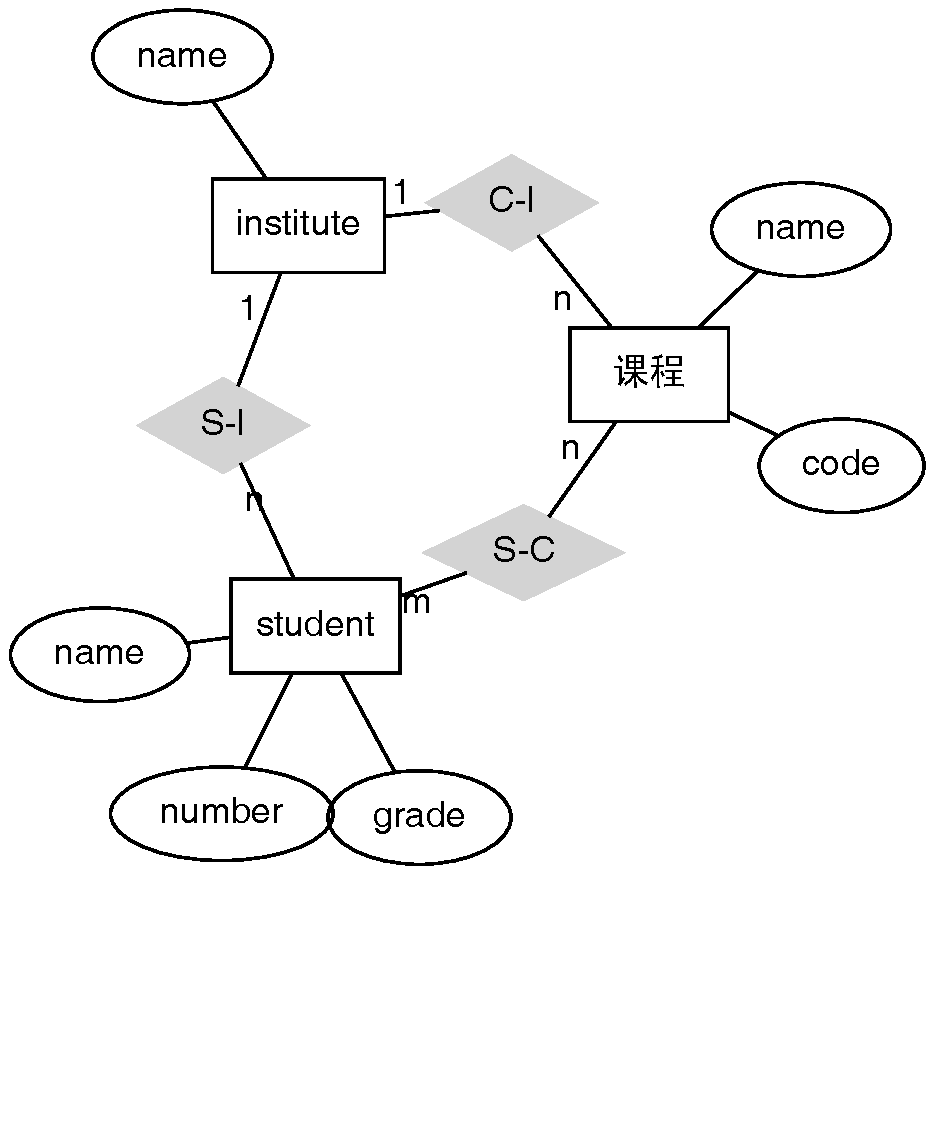
\includegraphics[width=0.8\textwidth]{svg/er_rsvg.pdf}
    \caption{inkscape转svgER图为pdf}
    \label{fig:svg_pdf_chocolatey}
\end{figure}
\section{插入算法}
\par 本模板支持使用更常用的algorithm2e\footnote{\url{http://mirrors.ctan.org/macros/latex/contrib/algorithm2e/doc/algorithm2e.pdf}}宏包插入算法,如\cref{alg:gcd}所示。
\begin{algorithm}[htbp]
    \caption{最大公约数}
    \label{alg:gcd}
    \begin{small}
        \SetAlgoLined
        \KwIn{Two positive integers $a$ and $b$}
        \KwOut{The greatest common divisor of $a$ and $b$}
        \While{$b \neq 0$}{
            $r \leftarrow a \bmod b$\;
            $a \leftarrow b$\;
            $b \leftarrow r$\;
        }
        \Return{$a$}\;
    \end{small}
\end{algorithm}
\section{插入代码}
\par 本模板支持插入代码,且可以对常用语言进行基本高亮。
\begin{lstlisting}[language=bash,label=code:bash]
# 查找运行的python命令
ps -ef | grep python
# 杀死全部占用某端口的程序
netstat -tunlp | grep $1 | awk '{print $7}' | tr '/' '\n' | head -n 1 | xargs kill -9
\end{lstlisting}
\par 本模板还支持插入外部代码。
\lstinputlisting[language=Perl,keywordstyle=\color{blue},commentstyle=\color{green},stringstyle=\color{red}]{example.pl}
